\documentclass[12pt,a4paper]{report}
\usepackage[left=2cm,right=2cm,top=2cm,bottom=2cm]{geometry}
\usepackage[onehalfspacing]{setspace}

\usepackage[T1]{fontenc}
\usepackage[utf8]{inputenc}
\usepackage[ngerman]{babel}
\usepackage{pifont}

\usepackage{graphicx}
\usepackage[export]{adjustbox}
\usepackage[hidelinks]{hyperref}
\usepackage{wrapfig}
\usepackage{mathtools}
\usepackage{listings}
\usepackage{multirow}
\usepackage{url}
\usepackage{pdfpages}
\usepackage{tabto}
\usepackage{tikz}
\usetikzlibrary{matrix,chains,positioning,decorations.pathreplacing,arrows,calc}
\usepackage{pgfplots}
\usepackage{amsmath}
\usepackage{subfig}

\graphicspath{{C:/Jetbrains/PyCharm/WerbeSkip/thoughts/arbeit/}}

\begin{document}

\begin{titlepage}
	\centering
	{\Large Gymnasium Bäumlihof, 5Bb \par}
	\vspace{1cm}
	{\LARGE\scshape Maturaarbeit\par}
	\vspace{1.5cm}
	{\huge\bfseries Kann der Computer Werbung erkennen?\par}
	\vspace{0.6cm}
    {\Large Bilderkennung mit einem neuronalen Netzwerk\par}
	\vspace{2cm}
	{\Large\itshape Georg Schwan\par}
	\vfill
	Betreuungsperson\par
	{\itshape Test1\par}
	Korreferent\par
	{\itshape Test2}
	\vfill
	{\large Basel, \today\par}
\end{titlepage}

\tableofcontents

\newpage

\chapter{Einleitung}\label{ch:einleitung}

\section{Motivation}
\label{sec:motivation}
Vor ein paar Jahren haben wir beim Fernsehen immer wenn Werbung kam den Sender gewechselt
bis die Werbung vorbei war und das normale Programm weiterlief.
Das Problem war nur, dass wir nie wussten, wann die Werbung vorbei war.
Meinem Bruder ist damals aufgefallen, dass bei Werbung nie das Logo vom Sender eingespielt wird.
Daraufhin hat er probiert ein Algorithmus zu schreiben, der das Logo vom Sender erkennen kann.
Er versuchte das Logo mithilfe von Bedingungen und Schleifen auszudrücken, aber es funktionierte nicht.

Als ich auf der Suche nach einer Idee für eine Maturaarbeit war, erinnerte ich mich wieder an das Problem und ich wählte einen neuen Lösungsansatz
nämlich neuronale Netzwerke, welche heute überall verwendet werden und extrem mächtig sind.
Die Idee war aber nicht nur ein Logo zu erkennen, sondern auch genau zu verstehen wie ein neuronales Netzwerk funktioniert und warum es so mächtig ist.
\section{Aufbau der Arbeit}
\label{sec:aufbauDerArbeit}
Im Abschnitt~\ref{sec:problemstellung} wird die genaue Problemstellung erklärt.
Im Kapitel~\ref{ch:neuronalesNetzwerk} wird das neuronale Netzwerke beschrieben.
Im Kapitel~\ref{ch:lösungsansatz} wird die Lösungsidee präsentiert.
Im Kapitel~\ref{ch:umsetzung} wird grob die Implementierung des neuronalen Netzwerkes beschrieben.
Im Kapitel~\ref{ch:ergebnisseUndAuswertung} werden die Ergebnisse der Netzwerke präsentiert und ausgewertet.
Im Kapitel~\ref{ch:fazitUndWeiterführung} ziehe ich ein Fazit und zeige mögliche Weiterführungen auf, die die Ergebnisse noch verbessern könnten.

\section{Einschränkung}
Neuronale Netzwerke sind ein sehr umfangreiches Thema und deswegen begrenze ich mich auf Netzwerke, die für die Bilderkennung entscheidend sind.
Darunter sind klassische feedforward und convolution Netzwerke.
Auf recurrent neuronale Netzwerke\footnote{Ein neuronales Netzwerk, das geeignet für Sequenzen ist\cite{wiki:rnn}} gehe ich nicht näher ein,
obwohl sie nützlich wären.

\section{Problemstellung}\label{sec:problemstellung}
Das Ziel dieser Arbeit ist einen Algorithmus zu programmieren, der Bilder als Werbung erkennen kann.
Dafür wird ein neuronales Netzwerk benutzt, das sich auf die Bilderkennung beschränkt.
\subsubsection{Logo}
Wie schon gesagt wird bei Werbung das Senderlogo nicht eingeblendet.
Deswegen kann das Problem vereinfacht werden auf die Frage,
ob das Senderlogo eingeblendet ist oder nicht (siehe Abbildung~\ref{fig:logo1}).
\begin{figure}[h]%
    \centering
    \subfloat[Werbung]{{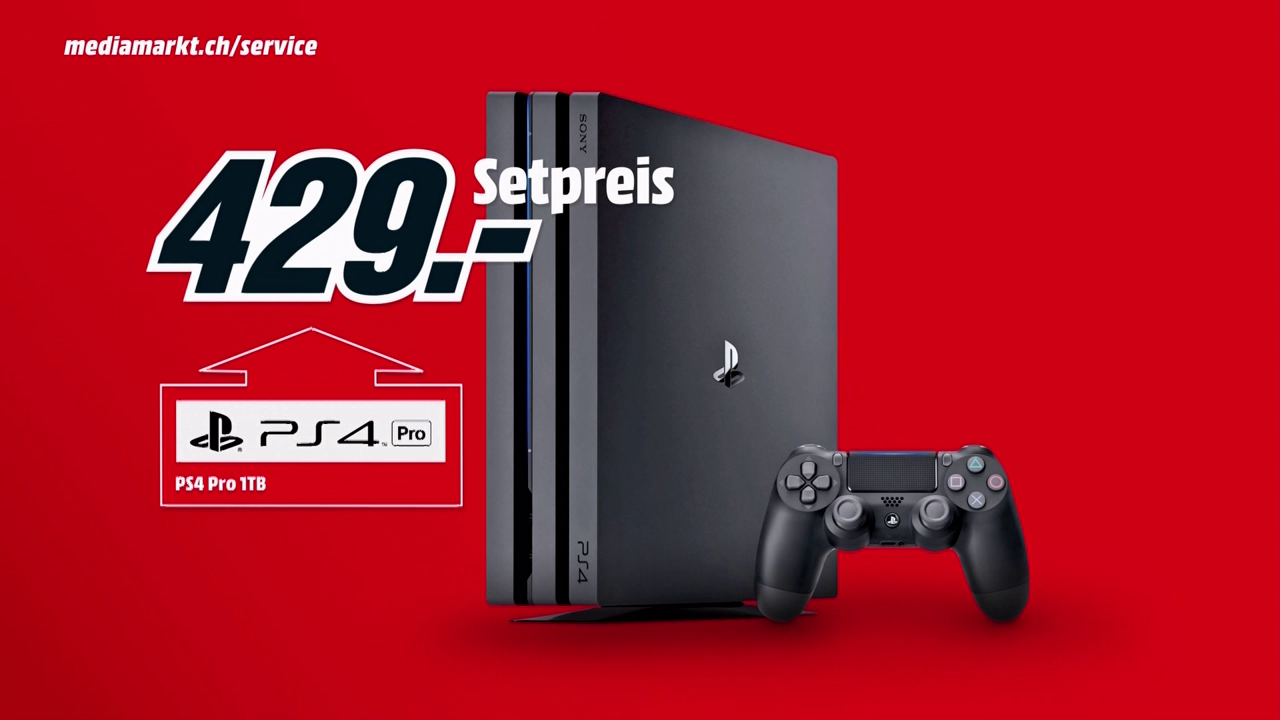
\includegraphics[width=7cm]{assets/images/prosieben_kein_logo.png} }}%
    \qquad
    \subfloat[Keine Werbung]{{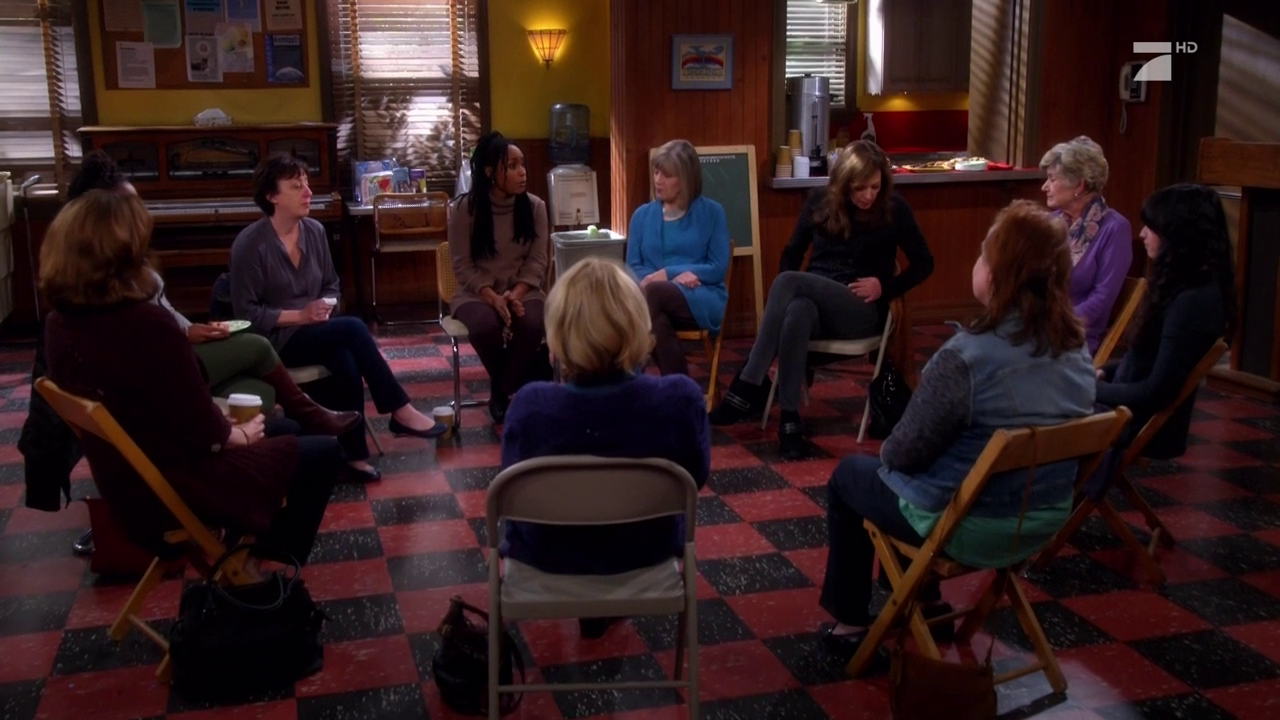
\includegraphics[width=7cm]{assets/images/prosieben_logo.png} }}%
    \caption{Kein Senderlogo bei Werbung}%
    \label{fig:logo1}%
\end{figure}
Man könnte meinen, dass das Erkennen eines Logos relativ simple ist.
Zum Beispiel könnte man überprüfen, ob der Bereich, wo das Logo sein sollte, heller ist als ausserhalb.

\begin{figure}[h]%
    \centering
    \subfloat[]{{
\includegraphics[width=3cm]{assets/images/logo_beispiel1.png} }}%
    \qquad
    \subfloat[]{{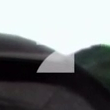
\includegraphics[width=3cm]{assets/images/logo_beispiel3.png} }}%
    \qquad
    \subfloat[]{{
\includegraphics[width=3cm]{assets/images/logo_beispiel4.png} }}%
    \qquad
    \subfloat[]{{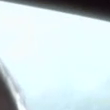
\includegraphics[width=3cm]{assets/images/logo_beispiel5.png} }}%
    \caption{Logo mit verschiedenen Hintergründen}%
    \label{fig:logo2}%
\end{figure}

Ein Problem des Logos ist, dass es nicht einfach über das normale Bild eingespielt wird, sondern dass man leicht hindurchsehen kann (siehe Abbildung~\ref{fig:logo2}a).
Dadurch kann das Logo nicht an gleichen Pixel erkannt werden.
Die grösste Schwierigkeit ist aber, dass bei manchen Hintergründen, vor allem bei Weissen, das Logo abgeschnitten oder kaum bis gar nicht sichtbar ist.
Bei Abbildung~\ref{fig:logo2} (b) ist das Logo abgeschnitten, bei (c) ist es kaum sichtbar und bei (d) ist komplett verschwunden.

Eine weitere Schwierigkeit ist, dass das Logo nicht unbedingt immer am gleichen Ort sein muss.
Zum Beispiel hat Prosieben 3 verschiedene Positionen (siehe Abbildung~\ref{fig:logo3}).
\begin{figure}[h]%
    \centering
    \subfloat[]{{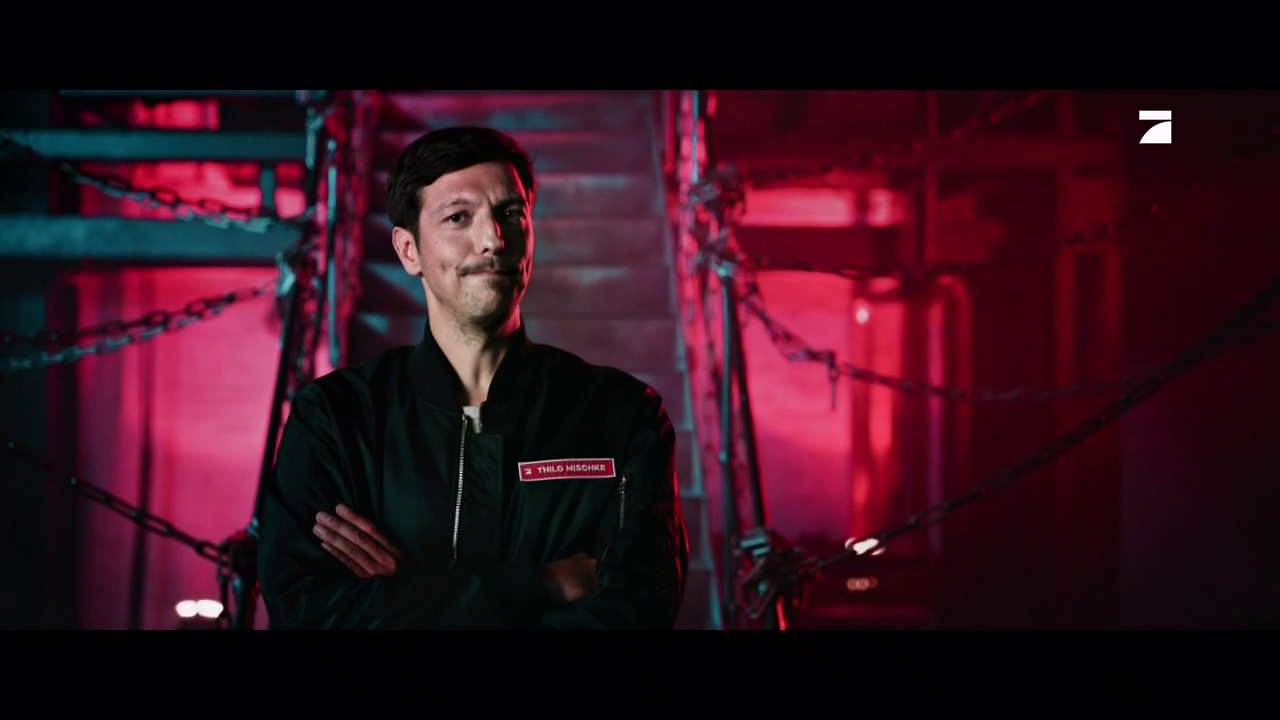
\includegraphics[width=6cm]{assets/images/logo_boarder_above.png} }}%
    \qquad
    \subfloat[]{{
\includegraphics[width=6cm]{assets/images/logo_boarder_side.png} }}%
    \qquad
    \subfloat[]{{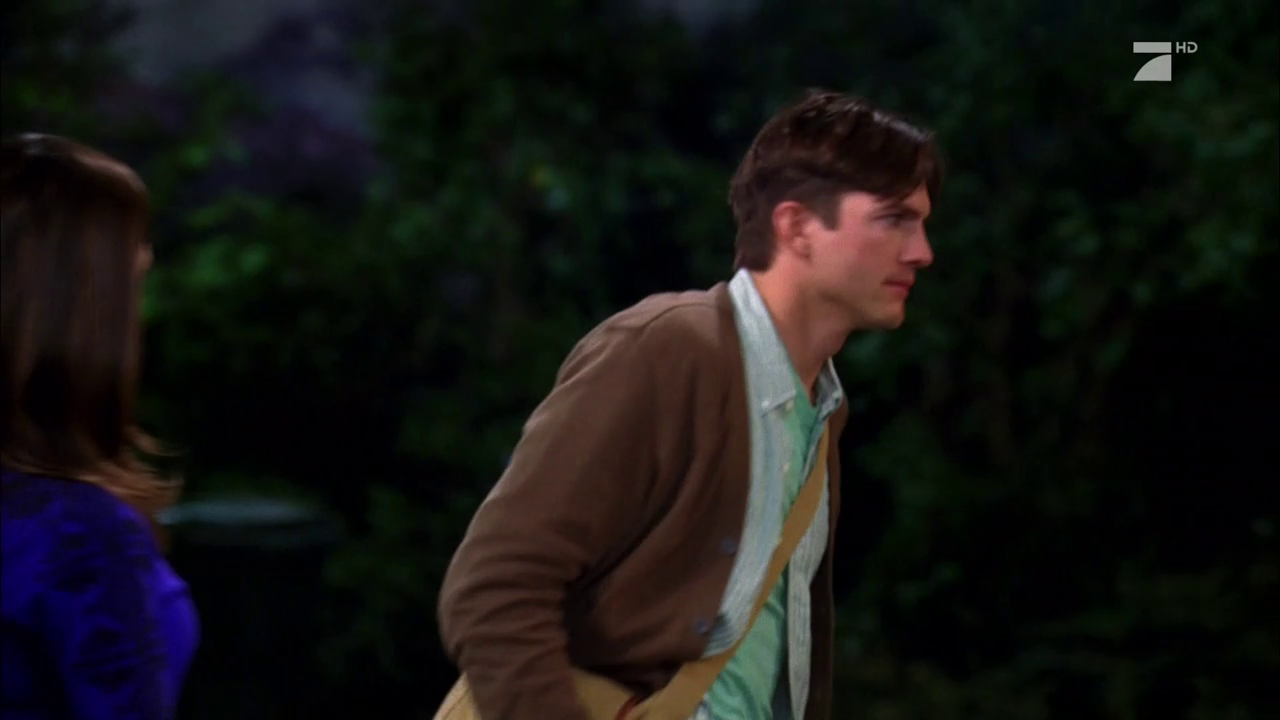
\includegraphics[width=6cm]{assets/images/logo_no_boarder.png} }}%
    \caption{Logo an verschiedenen Positionen}%
    \label{fig:logo3}%
\end{figure}
Alle diese Schwierigkeiten machen das Erkennen eines Logos ohne ein neuronales Netzwerk extrem schwierig.
Ein neuronales Netzwerk hingegen löst das Problem ziemlich elegant.

Eine weiter Frage, auf die eingegangen wird ist, ob ein neuronales Netzwerk auch ohne ein Logo Werbung erkennen kann.


\chapter{Neuronales Netzwerk}
\label{ch:neuronalesNetzwerk}
Dieses Kapitel bezieht sich auf das Buch von Michael A. Nielsen\cite{neuralbook}, ausser es wird anders angegeben.
\section{Konzept}\label{sec:konzept}
Wenn man ein normales Programm schreiben will, muss man das Problem in viele kleinere aufteilen, bis der Computer fähig ist,
es zu lösen.
In einem neuronalen Netzwerk wird dem Computer nicht gesagt wie es das Problem lösen kann, sondern ein neuronales Netzwerk
versteht das Problem, indem es Beispieldaten bekommt und an ihnen lernen kann, bis es seine eigene Lösung gefunden hat.
Zum Beispiel wollen wir einem Netzwerk beibringen, ob in einem Bild ein Auto vorkommt.
Dazu geben wir dem neuronalen Netzwerk viele Bilder, mit und ohne Auto.
Mit jedem Bild, dass das neuronale Netzwerk bekommt, lernt es besser wie ein Auto ausschaut.

Das Konzept eines neuronalen Netzwerks ist nicht etwas Neues.
Im Jahre 1957 hat Frank Rosenblatt eine erste Idee eines neuronalen Netzwerks vorgestellt.
Die Idee war, aus mathematischen Funktionen unser Gehirn zu modellieren,
indem man die biologischen Neuronen und Synapsen als mathematische Funktion ausdrückt.

Es ist aber erst in den letzen Jahren der grosse Hype auf neuronale Netzwerke ausgebrochen.
Dies liegt daran, dass man erst jetzt die nötigen Daten
und Rechenleistung zur Verfügung hat.

\section{Neuron}\label{sec:neuron}
User Gehirn kann Entscheidungen treffen, da wir Billionen von Neuronen haben, die miteinander verbunden sind und sich
verständigen können.
Ein Neuron an sich ist praktisch nutzlos, aber in grosser Anzahl können sie komplexeste Probleme lösen.

Nach dem gleichen Prinzip funktioniert ein neuronales Netzwerk,
Es besteht aus vielen Neuronen (daher der Name) die miteinander verbunden sind.


\begin{figure}[h]
    \centering
\begin{tikzpicture}[
init/.style={
  draw,
  circle,
  inner sep=2pt,
  font=\Huge,
  join = by -latex
},
squa/.style={
  draw,
  inner sep=2pt,
  font=\Large,
  join = by -latex
},
start chain=2,node distance=13mm
]
\node[on chain=2]
  (x2) {$x_2$};
\node[on chain=2,join=by o-latex]
  {$w_2$};
\node[on chain=2,init] (sigma)
  {$\displaystyle\Sigma$};
\node[on chain=2,squa,label=above:{\parbox{4cm}{\centering Aktivierungs-\\funktion}},join=by -latex, minimum size=0.9cm]
  {$f$};
\node[on chain=2,label=above:Ausgabe,join=by -latex]
  {$y$};
\begin{scope}[start chain=1]
\node[on chain=1] at (0,1.5cm)
  (x1) {$x_1$};
\node[on chain=1,join=by o-latex]
  (w1) {$w_1$};
\end{scope}
\begin{scope}[start chain=3]
\node[on chain=3] at (0,-1.5cm)
  (x3) {$x_3$};
\node[on chain=3,label=below:Gewichte,join=by o-latex]
  (w3) {$w_3$};
\end{scope}
\node[label=above:\parbox{2cm}{\centering Bias \\ $b$}] at (sigma|-w1) (b) {};

\draw[-latex] (w1) -- (sigma);
\draw[-latex] (w3) -- (sigma);
\draw[o-latex] (b) -- (sigma);

\draw[decorate,decoration={brace,mirror}] (x1.north west) -- node[left=10pt] {Eingabe} (x3.south west);
\end{tikzpicture}
    \caption{Einzelner Neuron in einem Neuronalen Netzwerks}
    \label{fig:neuron1}
\end{figure}

Ein Neuron in einem neuronalen Netzwerk wird als mathematische Funktion definiert wie Abbildung~\ref{fig:neuron1}
verdeutlicht.
Ein Neuron hat $n$ verschiedene Eingaben, die als $x_j$ bezeichnet werden und mit einem spezifischen Gewicht $w_j$ multipliziert werden.
Die Ausgabe erfolgt, indem man alle gewichteten Eingaben, mit einem Bias $b$, addiert und durch eine so genannte
Aktivierungsfunktion $f$ durchlaufen lässt.
Eine klassische Aktivierungsfunktion ist die Sigmoid Funktion $f(x) = \frac{1}{1 + e^{-x}}$, welche den Wert zwischen 0 und 1 normalisiert.
Als Gleichung:
\[y =f\left(\sum_{j=1}^{n} x_j w_j + b\right)\]
Die Gewichte $w_j$ und der Bias $b$ des Neurons sind die Parameter, die angepasst werden und somit das Neuron lernfähig machen.

Eine Aktivierungsfunktion ist nötig.
Ohne sie wäre ein neuronales Netzwerk eine komplett lineare Funktion,
welche nur lineare Probleme lösen könnte\cite{activations}, da in einem Netzwerk nur multipliziert und addiert wird.
Durch die Aktivierungsfunktion kommt eine nicht lineare Funktion hinzu, welche das Netzwerk komplizierter machen
aber auch mächtiger, da es so Beziehungen von Datenpunkten auch nicht linear miteinander Verknüpfen kann.
Ohne diese Aktivierungsfunktion wäre das Netzwerk nicht in der Lage komplizierte Zusammenhänge wie auf Bildern oder in der Sprache zu erkennen\cite{activations}.

Im Abschnitt~\ref{sec:aktivierungsfunktionen} wird näher auf die Aktivierungsfunktion eingegangen.

\section{Architektur}
Wie auch im biologischen Gehirn ist ein Neuron allein nutzlos.
Erst wenn man die Neuronen miteinander verbindet, kann es komplexe Zusammenhänge modellieren.
\begin{figure}[h]
    \centering
\begin{tikzpicture}[
plain/.style={
  draw=none,
  fill=none,
  },
net/.style={
  matrix of nodes,
  nodes={
    draw,
    circle,
    inner sep=10pt
    },
  nodes in empty cells,
  column sep=2cm,
  row sep=-9pt
  },
>=latex
]
\matrix[net] (mat)
{
|[plain]| \parbox{1.3cm}{\centering} & |[plain]| \parbox{1.3cm}{\centering} & |[plain]| \parbox{1.3cm}{\centering} \\
& |[plain]| \\
|[plain]| & \\
& |[plain]| \\
  |[plain]| & |[plain]| \\
& & \\
  |[plain]| & |[plain]| \\
& |[plain]| \\
  |[plain]| & \\
& |[plain]| \\    };
\foreach \ai [count=\mi ]in {2,4,...,10}
  \draw[<-] (mat-\ai-1) -- node[above] {Eingabe $x_\mi$} +(-2.8cm,0);
\foreach \ai in {2,4,...,10}
{\foreach \aii in {3,6,9}
  \draw[->] (mat-\ai-1) -- (mat-\aii-2);
}
\foreach \ai in {3,6,9}
  \draw[->] (mat-\ai-2) -- (mat-6-3);
\draw[->] (mat-6-3) -- node[above] {Ausgabe} +(2.5cm,0);
\end{tikzpicture}
    \caption{Mögliche Architektur eines neuronalen Netzwerk}
    \label{fig:network1}
\end{figure}

Eine mögliche Architektur kann wie in  Abbildung~\ref{fig:network1} ausschauen.
Ein Netzwerk wird generell immer in verschiedene Schichten unterteilt.
Die linke Schicht wird als eingabe Schicht bezeichnet und die Neuronen in dieser Schicht werden Eingabe Neuronen genannt.
Analog dazu wird die rechte Schicht Ausgabe Schicht genannt, die die Ausgabe Neuronen beinhaltet.
Die mittleren Schichten, die von der Anzahl her variieren können, werden versteckte Schichten genannt.
Die Anzahl der Neuronen in jeder Schicht kann auch variieren.
Abbildung~\ref{fig:network2} zeigt eine andere mögliche Architektur für ein Netzwerk, welche 2 versteckte
Schichten hat.
\begin{figure}[h]
    \centering
\begin{tikzpicture}[
plain/.style={
  draw=none,
  fill=none,
  },
net/.style={
  matrix of nodes,
  nodes={
    draw,
    circle,
    inner sep=10pt
    },
  nodes in empty cells,
  column sep=2cm,
  row sep=-9pt
  },
>=latex
]
\matrix[net] (mat)
{
|[plain]|  & |[plain]|  & |[plain]|  & |[plain]| \\
& |[plain]|& |[plain]|& |[plain]| \\
|[plain]| && |[plain]|& |[plain]| \\
& |[plain]|&& |[plain]|& |[plain]| \\
  |[plain]| && |[plain]|&& |[plain]| \\
& |[plain]| & \\
  |[plain]| && |[plain]|&& |[plain]| \\
& |[plain]| && |[plain]|& |[plain]|  \\
  |[plain]| & & |[plain]|& |[plain]|  \\
& |[plain]|& |[plain]|& |[plain]| \\     };
\foreach \ai in {2,4,...,10}
{\foreach \aii in {3,5, 7,9}
  \draw[->] (mat-\ai-1) -- (mat-\aii-2);
}
\foreach \ai in {3,5,7,9}
{\foreach \aii in {4,6,8}
  \draw[->] (mat-\ai-2) -- (mat-\aii-3);
}
\foreach \ai in {4,6,8}
{\foreach \aii in {5, 7}
  \draw[->] (mat-\ai-3) -- (mat-\aii-4);
}
\draw[decorate,decoration={brace}] (mat-1-1.west) -- node[above=5pt] {\parbox{3cm}{\centering Eingabe\\Schicht}} (mat-1-1.east);
\draw[decorate,decoration={brace}] (mat-1-2.west) -- node[above=5pt] {\parbox{3cm}{\centering Versteckte\\Schichten}} (mat-1-3.east);
\draw[decorate,decoration={brace}] (mat-1-4.west) -- node[above=5pt] {\parbox{3cm}{\centering Ausgabe\\Schicht}} (mat-1-4.east);
\draw[decorate,decoration={brace,mirror}] ($(mat-1-1.west)+(-0.1cm,-0.2cm)$) -- node[left=5pt] {\parbox{2cm}{\centering Eingabe\\Neuronen}} ($(mat-10-1.west) + (-0.1cm,-16pt)$);
\draw[decorate,decoration={brace}] ($(mat-5-4.east)+(+0.1cm,+16pt)$) -- node[right=5pt] {\parbox{2cm}{\centering Ausgabe\\Neuronen}} ($(mat-7-4.east) + (+0.1cm,-16pt)$);
\end{tikzpicture}
    \caption{Neuronales Netzwerk mit 2 versteckten Schichten}
    \label{fig:network2}
\end{figure}
Jedes Neuron der vorigen Schicht ist mit jedem Neuron der nachfolgenden Schicht verbunden,
welches als \textit{völlig verbundene Schicht} bezeichnet wird.
Dies ist ein klassisches feedforward Netzwerk,
welches nur Verbindungen nach vorne hat. So können keine Schleifen entstehen\footnote{Es gibt auch Architekturen, in denen Schleifen vorkommen,
aber auf diese wird nicht näher eingegangen}.

\subsubsection{Beschriftung}

Um eine allgemeine Gleichung zu bestimmen, muss man zuerst die Elemente des Netzwerks benennen.
Wir bezeichnen das Gewicht $w^l_{k,j}$\footnote{Das $l$ dient nur zur Indexierung und nicht als Potenz} für die Verbindung des $k^{ten}$ Neuron der $(l-1)^{ten}$ Schicht
zu dem $j^{ten}$ Neuron der $l^{ten}$ Schicht.
Ähnlich dazu bezeichnen wir die Ausgabe des Neurons als $a^l_j$ und der Bias des Neurons als $b^l_j$ (siehe Abbildung~\ref{fig:network3}).

\begin{figure}[h]
    \centering
\begin{tikzpicture}[
plain/.style={
  draw=none,
  fill=none,
  },
net/.style={
  matrix of nodes,
  nodes={
    draw,
    circle,
    inner sep=10pt
    },
  nodes in empty cells,
  column sep=2cm,
  row sep=-9pt
  },
>=latex
]
\matrix[net] (mat)
{
|[plain]| \parbox{2cm}{\centering Schicht 1} & |[plain]| \parbox{2cm}{\centering Schicht 2} & |[plain]| \parbox{2cm}{\centering Schicht 3} \\
& |[plain]| \\
|[plain]| \\
& &|[plain]| \\
  |[plain]| & |[plain]| \\
& & \\
  |[plain]| & |[plain]| \\
& &|[plain]| \\
  |[plain]| \\
& |[plain]| \\    };
\foreach \ai in {2,4,...,10}
{\foreach \aii in {4,6,8}
  \draw[->] (mat-\ai-1) -- (mat-\aii-2) coordinate[midway](center1\ai\aii);
}
\foreach \ai in {4,6,8}
  \draw[->] (mat-\ai-2) -- (mat-6-3) coordinate[midway](center2\ai);


\node[] at (mat-4-2)
  (x3) {$a^2_1$};
\node[] at (mat-6-2)
  (x3) {$a^2_2$};
\node[] at (mat-8-2)
  (x3) {$a^2_3$};
\node[] at (mat-6-3)
  (x3) {$a^3_1$};

\node (h1) at (-1.5, 2.2) {$w^2_{2,1}$};

\draw[->] (h1) -- (center144);

\node (h2) at (3, 1.5) {$w^3_{3,1}$};

\draw[->] (h2) -- (center28);

\end{tikzpicture}
    \caption{Bezeichnung der Parameter}
    \label{fig:network3}
\end{figure}
Mit dieser Notation kann eine Gleichung für das Netzwerk aufgestellt werden.

\[a^l_j = f\left(\sum_{k} a^{l-1}_k w^l_{k,j} + b^l_j\right)\]

\section{Wie das Netzwerk lernt}\label{sec:lernen}
Bis jetzt ging es nur darum wie ein neuronales Netzwerk aufgebaut ist.
In diesem Abschnitt bespreche ich, wie ein neuronales Netzwerk anhand von Daten lernen kann.
\subsection{Kostenfunktion}
Damit ein Netzwerk lernen kann, muss man dem Netzwerk zuerst sagen können wie gut oder wie schlecht es gerade ist.
Dazu definieren wir eine Kostenfunktion $C$, die von allen Gewichten $w$ und allen Biases $b$ abhängig ist.
Der Ausgabewert des kompletten Netzwerks wird als $y$ bezeichnet und die entsprechende gewünschte Ausgabe als $l$.
Dabei ist wichtig zu beachten, dass $y$ und $l$ Vektoren sind.
Zum Beispiel würde ein Bild, das 10x10 Pixel gross ist, als ein ($10 * 10 =$)100-dimensionaler Vektor dargestellt werden,
wobei jeder Eintrag im Vektor der Grauwert eines Pixels ist.
Die Dimension vom Ausgabe Vektor $y$ und des gewünschten Ausgabe Vektor $l$ entspricht der Anzahl Neuronen in der letzten Schicht des Netzwerks,
wobei jedes Neuron etwas bestimmtes aussagt.
Zum Beispiel könnte ein Neuron für das Vorkommen eines Autos im Bild stehen, wobei 0 für kein Auto und 1 für ein Auto steht.

\[C(w,b) = \sum_{j}(y_j - l_j)^2\]

Das Ziel des Netzwerkes ist diese Kostenfunktion zu minimieren, bis so viele Beispieldaten wie möglich $C \approx 0$ entsprechen,
dies geschieht, wenn die Ausgabe des Netzwerks und die gewünschte Ausgabe ähnlich ist.
\subsection{Gradient Descent}
Um diese Kostenfunktion zu minimieren wird ein Algorithmus namens \textit{gradient descent} benutzt.
Das Konzept basiert darauf, dass man eine Funktion, in Abhängigkeit einer Variablen ableiten kann und so die Steigung (eng. gradient)
an diesem Punkt berechnen kann und die Variable Richtung Minimum anpasst.

\begin{figure}[h]%
    \centering
    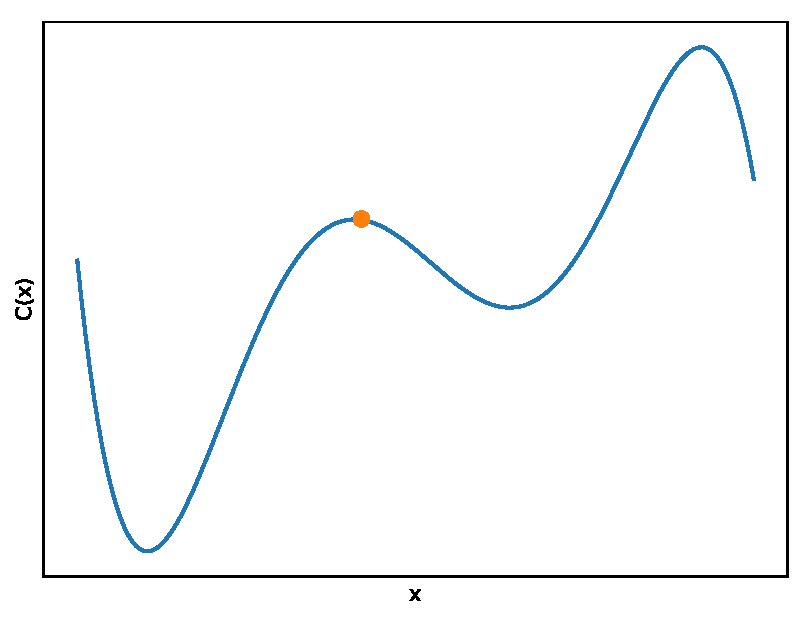
\includegraphics[width=10cm]{C:/Jetbrains/PyCharm/WerbeSkip/thoughts/arbeit/assets/python/gradient_empty.pdf} %
    \caption{Kostenfunktion in Abhängigkeit von $x$}%
    \label{fig:grad1}%
\end{figure}

Zum Beispiel hat man eine Kostenfunktion $C(x)$, die von $x$ abhängig ist (siehe Abbildung~\ref{fig:grad1}).

Die Variable $x$ wird am Anfang einem zufälligem Wert zugewiesen,
welcher dem orangen Punkt auf der Abbildung~\ref{fig:grad1} entspricht.
Das Ziel ist $s$ so anzupassen,
dass man ein Minimum der Kostenfunktion findet.
Um ein Minimum zu finden kann man sich einen Ball vorstellen, der in ein Minimum herunterrollt.
Um dies zu berechnen, muss man die Steigung mithilfe einer Ableitung herausfinden und die Variable in die
gegensätzliche Richtung bewegen.
\[a \rightarrow a^\prime\ = a - \eta\frac{\partial C}{\partial a}\]
wobei $\mu$ eine kleine positive Zahl (learning rate genannt) ist, die die Geschwindigkeit der Bewegung steuert.
Ausserdem ist zu beachten, dass der Ball keine Beschleunigung hat.
Wenn man diese Gleichung iterativ anwendend, gelangt man früher oder später zum lokalen Minimum der Kostenfunktion (siehe Abbildung~\ref{fig:grad2}).

\begin{figure}[h]%
    \centering
    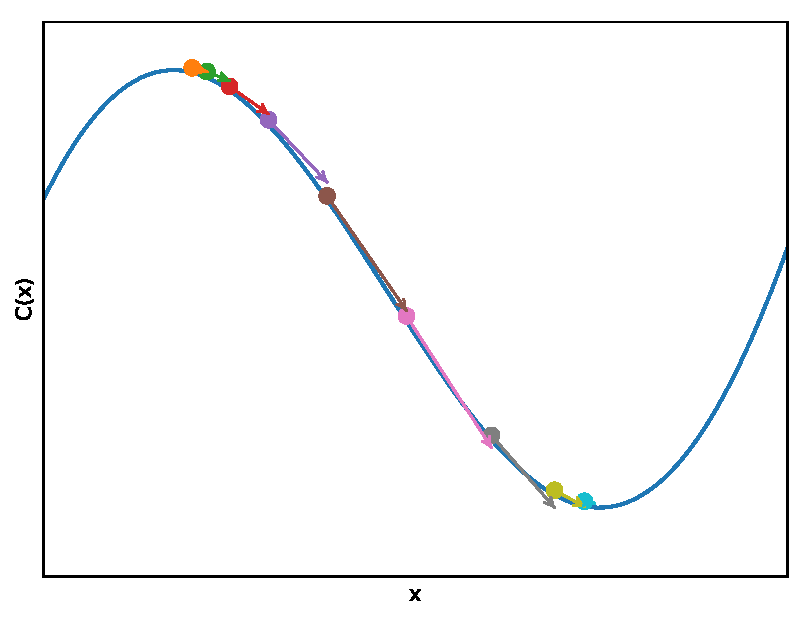
\includegraphics[width=10cm]{C:/Jetbrains/PyCharm/WerbeSkip/thoughts/arbeit/assets/python/gradient_full.pdf} %
    \caption{2-dimensionaler Verlauf des gradient descent}%
    \label{fig:grad2}%
\end{figure}

Der Algorithmus funktioniert auch bei mehr als nur einer Variable und lässt sich für die Gewichte und Biases des Netzwerkes genau gleich berechnen.
\begin{gather*}
    w^l_{k,j} \rightarrow w^{l^\prime}_{k,j} = w^l_{k,j} - \eta\frac{\partial C}{\partial w^l_{k,j}}\\
    b^l_j \rightarrow b^{l^\prime}_j = b^l_j - \eta\frac{\partial C}{\partial b^l_j}\\
\end{gather*}
Durch dieses Verfahren kann zwar relativ einfach ein Minimum gefunden werden, dabei ist aber zu beachten, dass es sich um ein lokales
Minimum handelt und nicht um ein globales.

\subsection{Backpropagation}
Den Algorithmus um $\frac{\partial C}{\partial w^l_{k,j}}$ und $\frac{\partial C}{\partial b^l_j}$ zu berechnen wird als
Backpropagation bezeichnet und ist der mathematisch schwerste Teil dieser Arbeit.
Es ist aber nicht unbedingt nötig für das Verständnis eines neuronalen Netzwerkes.
Es wird auch nicht näher auf die Beweise der Gleichungen eingegangen,
da es sonst zu kompliziert wird.
Im Grunde geht es nur um die Anwendung der Kettenregel.

Um die Übersicht zu behalten wird eine Zwischenmenge $\delta^l_j$ eingeführt, welches als \textit{Fehler} bezeichnet wird.
Der Fehler sagt aus, wie gut oder schlecht ein Neuron ist und ist definiert als:
\[\delta^l_j = \frac{\partial C}{\partial z^l_j}\]
wobei $z^l_j$ die Ausgabe von einem Neuron ohne die Aktivierungsfunktion ist, also $a^l_j = f(z^l_j)$.
Mit dieser Definition kann der Fehler in der letzten Schicht $L$ bestimmen werden:
\[\delta^L_j = \frac{\partial C}{\partial a^L_j}f^\prime(z^L_j)\]
%Der linke Teil $\frac{\partial C}{\partial a^L_j}$ gibt an wie schnell sich die Kosten in Abhängigkeit des $j^{ten}$ ausgang Neuron ändern.
%Der rechte Teil $f^\prime(z^L_j)$ zeigt wie schnell sich die Aktivierungsfunktion $f$ ändert bei $z^L_j$
In unserem Fall benutzen wir eine quadratische Kostenfunktion $C = \sum_{j}(a^L_j - y_j)^2$ bei
der die Ableitung $\frac{\partial C}{\partial a^L_j} = 2(a^L_j - y_j)$ ist und können $\delta^L_j$ einfacher definieren als:
\[\delta^L_j = 2(a^L_j - y_j)f^\prime(z^L_j)\]
Bei der Berechnung des Fehlers $\delta^l_j$ abhängig von $\delta^{l+1}_j$ bekommt man:
\[\delta^l_j = \sum_k w^{l+1}_{j,k}\delta^{l+1}_k f^\prime(z^l_j)\]
Es ist zu beachten, dass bei $w^{l+1}_{j,k}$ das $j$ und $k$ vertauscht sind, so dass man durch alle Neuronen der $(l+1)^{ten}$ Schicht durch iteriert.
Mit dieser Gleichung kann jeder Fehler von jeder Schicht berechnet werden, indem man von hinten durch das Netzwerk läuft.
Ähnlich wie wenn man sich beim Netzwerk nach vorne bewegt.

Die Gleichung für die Änderungsrate der Kosten in Bezug auf ein Bias im Netzwerk ist genau der Fehler:
\[\frac{\partial C}{\partial b^l_j} = \delta^l_j\]
Die Gleichung für die Änderungsrate der Kosten in Bezug auf ein Gewicht im Netzwerk ist:
\[\frac{\partial C}{\partial w^{l}_{k,j}} = a^{l-1}_k\delta^l_j\]

\section{Aktivierungsfunktionen}\label{sec:aktivierungsfunktionen}
Das einzige was jetzt noch fehlt ist wie eine Aktivierungsfunktion genau ausschaut.
Wie schon beschrieben darf eine Aktivierungsfunktion nicht linear sein, da sie sonst nichts neues zum Netzwerk beiträgt.
\subsection{Sigmoid}
Ein Beispiel für eine Aktivierungsfunktion ist die Sigmoid Funktion $f(x) = \frac{1}{1 + e^{-x}}$ (siehe Abbildung~\ref{fig:activation1}).
\begin{figure}[h]
    \centering
\begin{tikzpicture}
\begin{axis}[
    axis lines = left,
    xlabel = $x$,
    ylabel = {$f(x)$},
    ymin = -0.1,
    ymax = 1.1,
]
\pgfplotsset{
every axis legend/.append style={
at={(0.1,0.9)},
anchor=north west,
},
}
\addplot [
    domain=-8:8,
    samples=200,
    color=blue,
    ]
    {1 / (1 + 2.71828^(-x))};
\addlegendentry{$\frac{1}{1 + e^{-x}}$}

\end{axis}
\end{tikzpicture}
    \caption{Sigmoid Aktivierungsfunktionen}
    \label{fig:activation1}
\end{figure}
Besonders an dieser Funktion ist, dass sie den Ausgabewert zwischen 0 und 1 eingrenzt, was uns erlaubt den Ausgabewert des ganzen
Netzwerkes besser zu deuten, als wenn der Wert zwischen $-\infty$ und $\infty$ liegt.
Ein Problem der Sigmoid Funktion ist, dass wenn die Ausgabe nah bei 1 oder 0 ist, dann die Ableitung $f^\prime(x)$ davon auch nah bei 0 ist,
was den Fehler $\delta^l_j$ sehr klein hält und so das Netzwerk nur noch langsam lernen lässt.
Dieses Problem ist als \textit{vanishing gradient problem} bekannt.
\subsection{Rectified Linear Units}
Eine andere populäre Aktivierungsfunktion ist die Rectified linear units Funktion oder kurz ReLu.
\begin{figure}[h]
    \centering
\begin{tikzpicture}
\begin{axis}[
    axis lines = left,
    xlabel = $x$,
    ylabel = {$f(x)$},
    ymin = -2,
]
\pgfplotsset{
every axis legend/.append style={
at={(0.1,0.9)},
anchor=north west,
},
}
\addplot [
    domain=-8:8,
    samples=200,
    color=blue,
    ]
    {max(x, 0))};
\addlegendentry{$\max(0, x)$}

\end{axis}
\end{tikzpicture}
    \caption{ReLu Aktivierungsfunktionen}
    \label{fig:activation2}
\end{figure}
Die Funktion $f(x) = \max(0, x)$ (siehe Abbildung~\ref{fig:activation2}) löst das Problem des vanishing gradient.
Praktisch alle Neuronalen Netzwerke benutzen Relu als ihre Aktivierungsfunktion,
da es die besten Ergebnisse erbringt\cite{activations}.
Ein Nachteil ist, dass sie nur in den Versteckten Schichten gut funktioniert,
da der Ausgabewert der Funktion unendlich gross sein kann.
\subsection{Softmax}
Die softmax Funktion wird verwendet, um eindeutige Klassifikationen zu machen und ist definiert als:
\[f(x_j) = \frac{e^{x_j}}{\sum_k{e^{x_k}}}\]
Das besondere an dieser Aktivierungsfunktion ist, dass sie nicht nur einen Wert braucht, sondern alle Werte der ganzen Schicht,
d.h nicht nur ein $x_j$ sondern alle.
Ausserdem gibt die Summe aller Resultate $\sum_j f(x_j) = 1$ und kann deswegen als eine Wahrscheinlichkeitsverteilung verstanden werden.
Dies ist oft sehr hilfreich, da viele Probleme nur ein richtiges Resultat haben, zum Beispiel hat man Bilder von Zahlen,
wo immer nur eine Zahl pro Bild zu sehen ist.
Durch die softmax Funktion sieht man dann eine geschätzte Wahrscheinlichkeit vom Netzwerk für jede Zahl.
\section{Convolution}
Bis jetzt ging es nur um Schichten, die völlig miteinander verbunden sind.
Für die Bilderkennung kann das suboptimal sein, da bestimmte Eigenschaften eines Bildes nicht miteinbezogen werden,
wie zum Beispiel die Beziehung von nebeneinander liegenden Pixel.
Ausserdem kann das gesuchte Objekt in einem Bild an verschiedenen Orten vorkommen.
\subsection{Architektur}
Die Eingabe für einen convolutional Schicht ist nicht 1-dimensional, sondern 2-dimensional (siehe Abbildung~\ref{fig:conv1}).
\begin{figure}[h]
    \centering
\begin{tikzpicture}[
plain/.style={
  draw=none,
  fill=none,
  },
net/.style={
  matrix of nodes,
  nodes={
    draw,
    circle,
    inner sep=5pt
    },
  nodes in empty cells,
  column sep=2pt,
  row sep=2pt
  },
>=latex
]
\matrix[net] (mat)
{
|[plain]|  & |[plain]|  & |[plain]|  & |[plain]| & |[plain]|  & |[plain]| & |[plain]|\\
&  &   &  &  &  &  &  &  & \\
&  &   &  &  &  &  &  &  & \\
&  &   &  &  &  &  &  &  & \\
&  &   &  &  &  &  &  &  & \\
&  &   &  &  &  &  &  &  & \\
&  &   &  &  &  &  &  &  & \\
&  &   &  &  &  &  &  &  & \\
&  &   &  &  &  &  &  &  & \\
&  &   &  &  &  &  &  &  & \\
&  &   &  &  &  &  &  &  & \\
};
\node[] at (mat-1-6.north west)
  (x) {\centering Eingabe Neuronen};
\end{tikzpicture}
    \caption{Eingabe Neuronen für eine convolution Schicht}
    \label{fig:conv1}
\end{figure}
Die Neuronen werden normal verbunden einfach mit dem Unterschied, dass nicht jedes Neuron mit jedem Neuron verbunden wird,
sondern dass nur ein bestimmter Bereich zum nächsten Neuron verbunden ist.
Dieser Bereich wird als \textit{Filter} bezeichnet und in dem Beispiel auf Abbildung~\ref{fig:conv2} wird ein 3x3 Filter benutzt.
\begin{figure}[h]
    \centering
\begin{tikzpicture}[
plain/.style={
  draw=none,
  fill=none,
  },
net/.style={
  matrix of nodes,
  nodes={
    draw,
    circle,
    inner sep=5pt
    },
  nodes in empty cells,
  column sep=2pt,
  row sep=2pt
  },
>=latex
]
\matrix[net] (mat)
{
|[plain]|  & |[plain]|  & |[plain]|  & |[plain]| & |[plain]|  & |[plain]| & |[plain]|\\
&  &   &  &  &  &  &  &  &  &|[plain]|  & |[plain]|  & |[plain]|  & |[plain]| \\
&  &   &  &  &  &  &  &  &  &|[plain]|  & |[plain]|  & |[plain]|  & |[plain]| \\
&  &   &  &  &  &  &  &  &  &|[plain]|  & |[plain]|  & |[plain]|  & |[plain]| & |[plain]|\\
&  &   &  &  &  &  &  &  &  &|[plain]|  & |[plain]|  & |[plain]|  & |[plain]| & |[plain]|\\
&  &   &  &  &  &  &  &  &  &|[plain]|  & |[plain]|  & |[plain]|  & |[plain]| &\\
&  &   &  &  &  &  &  &  &  &|[plain]|  & |[plain]|  & |[plain]|  & |[plain]| \\
&  &   &  &  &  &  &  &  &  &|[plain]|  & |[plain]|  & |[plain]|  & |[plain]| \\
&  &   &  &  &  &  &  &  &  &|[plain]|  & |[plain]|  & |[plain]|  & |[plain]| \\
&  &   &  &  &  &  &  &  &  &|[plain]|  & |[plain]|  & |[plain]|  & |[plain]| \\
&  &   &  &  &  &  &  &  &  &|[plain]|  & |[plain]|  & |[plain]|  & |[plain]| \\
};
\node[] at (mat-1-6.north)
  (x) {\centering Eingabe Neuronen};

\node[] at (mat-5-15.north)
  (y) {\centering Verstecktes Neuron};

\foreach \ai in {7,...,9}
{\foreach \aii in {7,...,9}
  \node[circle, line width=1.5pt, draw, inner sep=5pt] at (mat-\ai-\aii) {};
}
\foreach \ai in {7,...,9}
{\foreach \aii in {7,...,9}
  \draw[->] (mat-\ai-\aii) -- (mat-6-15);
}
\end{tikzpicture}
    \caption{Verbindung eines versteckten Neurons in einem convolution Schicht}
    \label{fig:conv2}
\end{figure}
Der Filter wird dann auf den Eingabe Neuronen um ein Neuron verschoben, um den nächsten Neuron zu verbinden.
Und so geht das weiter, auch nach unten, bis die ganze versteckte Schicht gemacht wurde.
Dabei wird die versteckte Schicht auch kleiner (in dem Beispiel wird die 10x10 Schicht zu einer 8x8 Schicht),
da der Filter irgendwann am anderen Rand anstösst.
Abbildung~\ref{fig:conv3} verdeutlicht das Prinzip noch einmal.

Der Filter kann auch um mehr als nur einen Neuronen verschoben werden und man kann in den beiden Richtungen verschiedene Schrittweiten nehmen,
zum Beispiel bewegt sich der Neuron nach links um zwei Neuronen und nach unten um drei.
\begin{figure}[h]
    \centering
    \begin{tikzpicture}[
plain/.style={
  draw=none,
  fill=none,
  },
net/.style={
  matrix of nodes,
  nodes={
    draw,
    circle,
    inner sep=3pt
    },
  nodes in empty cells,
  column sep=1pt,
  row sep=1pt
  },
>=latex
]
\matrix[net] (mat)
{
|[plain]|  & |[plain]|  & |[plain]|  & |[plain]| & |[plain]|  & |[plain]| & |[plain]|  & |[plain]|  & |[plain]|  & |[plain]| & |[plain]|  & |[plain]| & |[plain]|& |[plain]|  & |[plain]|  & |[plain]|  & |[plain]|  & |[plain]|  \\
&  &   &  &  &  &  &  &  &  &|[plain]|  & |[plain]|  & |[plain]|  & |[plain]| \\
&  &   &  &  &  &  &  &  &  &|[plain]|  & |[plain]|  & |[plain]|  & |[plain]| &  &   &  &  &  &  & &\\
&  &   &  &  &  &  &  &  &  &|[plain]|  & |[plain]|  & |[plain]|  & |[plain]| &  &   &  &  &  &  & &\\
&  &   &  &  &  &  &  &  &  &|[plain]|  & |[plain]|  & |[plain]|  & |[plain]| &  &   &  &  &  &  & &\\
&  &   &  &  &  &  &  &  &  &|[plain]|  & |[plain]|  & |[plain]|  & |[plain]| &  &   &  &  &  &  & &\\
&  &   &  &  &  &  &  &  &  &|[plain]|  & |[plain]|  & |[plain]|  & |[plain]| &  &   &  &  &  &  & &\\
&  &   &  &  &  &  &  &  &  &|[plain]|  & |[plain]|  & |[plain]|  & |[plain]| &  &   &  &  &  &  & &\\
&  &   &  &  &  &  &  &  &  &|[plain]|  & |[plain]|  & |[plain]|  & |[plain]| &  &   &  &  &  &  & &\\
&  &   &  &  &  &  &  &  &  &|[plain]|  & |[plain]|  & |[plain]|  & |[plain]| &  &   &  &  &  &  & &\\
&  &   &  &  &  &  &  &  &  &|[plain]|  & |[plain]|  & |[plain]|  & |[plain]| \\
};
\node[] at (mat-1-6.north)
  (x) {\centering Eingabe Neuronen};

\node[] at (mat-1-18.north east)
  (y) {\centering Versteckte Schicht};

\foreach \ai in {2,...,4}
{\foreach \aii in {1,...,3}
  \node[circle, line width=1pt, draw, inner sep=3pt] at (mat-\ai-\aii) {};
}
\foreach \ai in {2,...,4}
{\foreach \aii in {1,...,3}
  \draw[->] (mat-\ai-\aii) -- (mat-3-15);
}

\end{tikzpicture}
    \hspace{0.5cm}% NO SPACE!
    \begin{tikzpicture}[
plain/.style={
  draw=none,
  fill=none,
  },
net/.style={
  matrix of nodes,
  nodes={
    draw,
    circle,
    inner sep=3pt
    },
  nodes in empty cells,
  column sep=1pt,
  row sep=1pt
  },
>=latex
]
\matrix[net] (mat)
{
|[plain]|  & |[plain]|  & |[plain]|  & |[plain]| & |[plain]|  & |[plain]| & |[plain]|  & |[plain]|  & |[plain]|  & |[plain]| & |[plain]|  & |[plain]| & |[plain]|& |[plain]|  & |[plain]|  & |[plain]|  & |[plain]|  & |[plain]|  \\
&  &   &  &  &  &  &  &  &  &|[plain]|  & |[plain]|  & |[plain]|  & |[plain]| \\
&  &   &  &  &  &  &  &  &  &|[plain]|  & |[plain]|  & |[plain]|  & |[plain]| &  &   &  &  &  &  & &\\
&  &   &  &  &  &  &  &  &  &|[plain]|  & |[plain]|  & |[plain]|  & |[plain]| &  &   &  &  &  &  & &\\
&  &   &  &  &  &  &  &  &  &|[plain]|  & |[plain]|  & |[plain]|  & |[plain]| &  &   &  &  &  &  & &\\
&  &   &  &  &  &  &  &  &  &|[plain]|  & |[plain]|  & |[plain]|  & |[plain]| &  &   &  &  &  &  & &\\
&  &   &  &  &  &  &  &  &  &|[plain]|  & |[plain]|  & |[plain]|  & |[plain]| &  &   &  &  &  &  & &\\
&  &   &  &  &  &  &  &  &  &|[plain]|  & |[plain]|  & |[plain]|  & |[plain]| &  &   &  &  &  &  & &\\
&  &   &  &  &  &  &  &  &  &|[plain]|  & |[plain]|  & |[plain]|  & |[plain]| &  &   &  &  &  &  & &\\
&  &   &  &  &  &  &  &  &  &|[plain]|  & |[plain]|  & |[plain]|  & |[plain]| &  &   &  &  &  &  & &\\
&  &   &  &  &  &  &  &  &  &|[plain]|  & |[plain]|  & |[plain]|  & |[plain]| \\
};
\node[] at (mat-1-6.north)
  (x) {\centering Eingabe Neuronen};

\node[] at (mat-1-18.north east)
  (y) {\centering Versteckte Schicht};

\foreach \ai in {2,...,4}
{\foreach \aii in {2,...,4}
  \node[circle, line width=1pt, draw, inner sep=3pt] at (mat-\ai-\aii) {};
}
\foreach \ai in {2,...,4}
{\foreach \aii in {2,...,4}
  \draw[->] (mat-\ai-\aii) -- (mat-3-16);
}

\end{tikzpicture}
    \caption{Bewegung eines Filters über eine convolution Schicht}
    \label{fig:conv3}
\end{figure}

Das Entscheidende am Filter ist, dass er die gleichen Gewichte und Bias verwendet für die Verbindung, d.h bei einem
Filter von 5x5 gibt is $(5*5=)$25 verschiedene Gewichte und einen Bias.
Wenn der Filter bewegt wird werden immer die gleichen Gewichte und der der gleiche Bias verwendet.
Als Gleichung bei einem 3x3 Filter:

\[a^{l+1}_{j,k} = f\left(\sum_{p=0}^{2}\sum_{m=0}^{2}w^l_{p,m}a^l_{j+p,k+m} + b^l\right)\]

wobei $a_{x, y}$ der Neuron an der Position $x, y$ ist und $f$ eine Aktivierungsfunktion.
Dadurch dass immer die gleichen Gewichte und der gleiche Bias für jeden Filter benutzt werden,
wird überall das gleiche Merkmal erkannt, auch wenn es sich an einem anderen Ort befindet.
Deswegen wird die Ausgabe von dem Filter als \textit{feature map} bezeichnet.
Normalerweise will man mehr als nur ein Merkmal erkennen und deswegen werden mehrere Filter verwendet,
wodurch mehrere feature maps entstehen (siehe Abbildung~\ref{fig:conv4}).
Der Grund warum die Filter nicht alle das gleiche Merkmal erkennen, liegt an der zufälligen Initialisierung der Gewichte und Biases.

Falls eine vor eine convolution  Schicht mehrer feature maps sind, würde der Bereich eines Filters alle feature maps beinhalten,
so dass ein Neuron mit einem Bereich von jeder feature map verbunden ist.
Man kann es sich so vorstellen, als ob der Filter in der Z-Achse erweitert würde.
Dadurch können auch relativ einfach farbige Bilder als Eingabe dienen,
da dann die eingabe Schicht einfach aus drei feature maps bestehen würde, da ein farbiges Bild aus drei Farbkanälen besteht.

\begin{figure}[h]%
    \centering
\begin{tikzpicture}
\draw [draw=black] (5,5.5) rectangle (0,0.5);
\draw [draw=black] (12,5) rectangle (7,0);
\draw [draw=black] (12.5,5.5) rectangle (7.5,0.5);
\draw [draw=black] (13,6) rectangle (8,1);
\draw[->] (5, 3) -- (7, 2.5);
\draw[->] (5, 3) -- (7.5, 3);
\draw[->] (5, 3) -- (8, 3.5);
\node[] at (2.5, 6.5)
  (y) {\centering Eingabe Schicht};

\node[] at (10, 6.5)
  (y) {\centering Versteckte Schicht};

\end{tikzpicture}
    \caption{Convolution Schicht mit 3 feature maps}%
    \label{fig:conv4}
\end{figure}

\subsection{Max Pooling}
Neben den convolution Schichten gibt es auch die maxpool Schicht\footnote{Es gibt noch andere pooling Schichten, die aber in dieser Arbeit nicht verwendet wurden},
die Idee vom Pooling ist, dass es die Informationen zusammenfasst.

Max polling nimmt eine feature map als Eingabe und lässt auch etwas Ähnliches wie ein Filter darüber laufen.
Der Filter bewegt sich genau gleich wie ein normaler mit dem Unterschied dass es keine lernbaren Parameter hat und
die Ausgabe des Filters der grösste Wert von den Eingaben ist (siehe Abbildung~\ref{fig:pool1}).
Ausserdem kann max pooling nur auf eine feature map angewendet werden,
d.h der max pool Filter hat keine Z-Achse und kann sich nur mit einzelne feature maps verbinden\cite{conv}.
\begin{figure}[h]
    \centering
    \begin{tikzpicture}[
plain/.style={
  draw=none,
  fill=none,
  },
net/.style={
  matrix of nodes,
  nodes={
    draw,
    circle,
    inner sep=10pt
    },
  nodes in empty cells,
  column sep=2pt,
  row sep=2pt
  },
>=latex
]
\matrix[net] (mat)
{
|[plain]|  & |[plain]|  & |[plain]|  & |[plain]| & |[plain]|  & |[plain]|  & |[plain]| \\
&  &   &  &  |[plain]|  & |[plain]|\\
&  &   &  &  |[plain]|  & |[plain]|\\
&  &   &  &  |[plain]|  & |[plain]| &  &  \\
&  &   &  &  |[plain]|  & |[plain]| &  &   \\
};
\node[] at (mat-1-2.east)
  (x) {\centering Feature Map};
\node[] at (mat-2-1)
  (y) {\centering 1};
\node[] at (mat-2-2)
  (y) {\centering 2};
\node[] at (mat-3-2)
  (y) {\centering 3};
\node[] at (mat-3-1)
  (y) {\centering 4};

\node[] at (mat-4-7)
  (y) {\centering 4};

\foreach \ai in {2,...,3}
{\foreach \aii in {1,...,2}
  \node[circle, line width=1pt, draw, inner sep=10pt] at (mat-\ai-\aii) {};
}
\foreach \ai in {2,...,3}
{\foreach \aii in {1,...,2}
  \draw[->] (mat-\ai-\aii) -- (mat-4-7);
}
\end{tikzpicture}
    \caption{2x2 maxpool Schicht mit einer Schrittweite von 2}
    \label{fig:pool1}
\end{figure}
Man kann max pooling verstehen als eine Reduzierung der vorhanden Informationen.
Es nimmt das wichtigste Merkmal in einem gewissen Bereich und wirft die weniger wichtigeren Merkmale weg,
so dass es weniger Neuronen gibt und die darauffolgenden Neuronen es einfacher haben.

\subsection{Convolution und Völlig Verbundene Schichten}
Um das Netzwerk zu interpretieren muss man eine völlig verbundene Schicht am Schluss haben,
da man eine 2-dimensionale Schicht sonst nicht interpretieren kann.\footnote{Es gibt Netzwerke, bei denen es eine convolution Schicht als Ausgabeschicht hat\cite{fullconvolution}}
Die völlig verbundene Schicht wird angehängt, indem jedes Neuron von der convolution bzw. maxpool Schicht mit jedem Neuron der völlig verbundenen Schicht verbunden wird.
Es spielt keine Rolle, dass die Neuronen 2-dimensional angeordnet sind.

Ausserdem ist das Trainieren des Netzwerks immer noch genau gleich.
Es wird immer noch gradient descent und backpropagation benutzt,
allerdings müssen die Gleichungen der backpropagation für die convolution und das max pooling angepasst werden.

\section{Regularization}
Um ein Netzwerk zu trainieren hat man meisten nur eine endliche Anzahl an Daten an denen das Netzwerk lernen kann.
Aus dem Grund werden die gleichen Daten mehrmals zum Trainieren verwendet.
Dadurch kann ein Problem entstehen:
Mit der Zeit kennt das Netzwerk die Trainingsdaten so gut, dass es die Trainingsdaten einfach auswendig lernt
und die Daten nicht mehr an ihren gemeinsamen Merkmalen und Zusammenhängen erkennt,
sondern an ihren ganz spezifischen Merkmalen die nur für die Trainingsdaten zutreffen.
Dadurch werden unbekannte Daten nicht mehr richtig erkannt.
Dieses Phänomen ist als \textit{overfitting} bekannt.
\subsection{Dropout}
Beim Trainieren eines Netzwerkes werden Neuronen mit einer bestimmten Wahrscheinlichkeit temporär deaktiviert bzw. ignoriert (siehe Abbildung~\ref{fig:dropout1}).
Bei jeder neuen Eingabe zum Trainieren werden neue zufällige Neuronen ausgewählt,
dabei sind die eingabe und ausgabe Neuronen davon ausgenommen.

\begin{figure}[h]
    \centering
\begin{tikzpicture}[
plain/.style={
  draw=none,
  fill=none,
  },
net/.style={
  matrix of nodes,
  nodes={
    draw,
    circle,
    inner sep=10pt
    },
  nodes in empty cells,
  column sep=2cm,
  row sep=-9pt
  },
>=latex
]
\matrix[net] (mat)
{
|[plain]|  & |[plain]|  & |[plain]|   \\
& |[plain]|& |[plain]|  \\
|[plain]| &|[plain]|& |[plain]|  \\
& |[plain]|&& |[plain]| \\
  |[plain]| && |[plain]|& \\
& |[plain]| & \\
  |[plain]| && |[plain]| & \\
& |[plain]| &|[plain]|& |[plain]|  \\
  |[plain]| & |[plain]|& |[plain]|  \\
& |[plain]|& |[plain]|  \\     };
\foreach \ai in {2,4,...,10}
{\foreach \aii in {5, 7}
  \draw[->] (mat-\ai-1) -- (mat-\aii-2);
}
\foreach \ai in {5,7}
{\foreach \aii in {4,6,8}
  \draw[->] (mat-\ai-2) -- (mat-\aii-3);
}
\foreach \ai in {4,6}
{\foreach \aii in {5, 7}
  \draw[->] (mat-\ai-3) -- (mat-\aii-4);
}

\node[circle, draw,dotted, inner sep=10pt] at (mat-3-2) {};
\node[circle, draw,dotted, inner sep=10pt] at (mat-9-2) {};
\node[circle, draw,dotted, inner sep=10pt] at (mat-8-3) {};

\foreach \ai in {2,4,...,10}
{\foreach \aii in {3,9}
  \draw[->, dotted] (mat-\ai-1) -- (mat-\aii-2);
  \
}
\foreach \ai in {3,9}
{\foreach \aii in {4,6,8}
  \draw[->, dotted] (mat-\ai-2) -- (mat-\aii-3);
}
\foreach \ai in {8}
{\foreach \aii in {5, 7}
  \draw[->, dotted] (mat-\ai-3) -- (mat-\aii-4);
}

\end{tikzpicture}
    \caption{neuronales Netzwerk mit Dropout}
    \label{fig:dropout1}
\end{figure}

Damit werden bestimmte Gewichte und Biases gelernt,
welche davon ausgehen, dass immer ein Teil der Neuronen nicht vorhanden ist.
Aber nach dem Training wird der Dropout nicht mehr benutzt und dadurch werden mehr Neuronen gleichzeitig aktiv sein als während dem Trainieren.
Um das aus zu gleichen wird die Ausgabe des Neurons mit der Wahrscheinlichkeit, mit der es deaktiviert wird, multipliziert.

Dropout hilft gegen overfitting,
da ein Neuron sich nicht auf andere Neuronen verlassen kann.
Dadurch ist es gezwungen mit vielen zufälligen Verbindungen etwas Nützliches anzufangen.
Anders gesagt: Das Netzwerk wird robust gegen den Verlust von einzelnen Merkmalen, da es sich nicht auf einzelne Merkmale verlassen kann.

\subsection{Batch Normalization}
Eine weitere Methode um overfitting zu vermeiden ist die \textit{Batch Normalization}.
Bei der Batch Normalization werden die Ausgaben der versteckten Schichten normalisiert\cite{batchnorm}.
so dass in den versteckten Schichten extreme Werte vermieden werden\cite{batchnorm}.
Ähnlich wie bei Dropout bringt Batch Normalization eine leichte Störung in das Netzwerk,
welches gegen overfitting hilft\cite{batchnorm}

Die Schichten werden normalisiert, indem beim Trainieren mehrere Eingaben gleichzeitig durch das Netzwerk laufen.
Die Ausgaben eines Neurones werden mit dem Mittelwert der Ausgaben subtrahieren und mit der
Standardabweichung der Ausgaben dividieren\cite{batchnorm}.
\begin{gather*}
    \mu = \frac{1}{m}\sum^m_{i=1}x_{i}\\
    \sigma = \frac{1}{m}\sum^m_{i=1}(x_i - \mu)^2\\
    \hat{x_i} = \frac{x_i - \mu}{\sqrt{\sigma}}\\
\end{gather*}
wobei $x_i$ die $i^{te}$ Ausgabe eines Neurons ist.

Ausserdem wird danach noch mit einem bestimmten Wert $\gamma_i$ multipliziert und einem bestimmten Wert $\beta_i$ addiert.
\[y_i = \gamma_i * \hat{x_i} + \beta_i \]
wobei $\gamma_i$ und $\beta_i$ Parameter sind, die beim Netzwerk trainiert werden wie ein normales Gewicht oder Bias\cite{batchnorm}.
Die Parameter werden benutzt um dem Netzwerk die Option zu geben die Normalisierung zu verändern oder sogar rückgängig zu machen, wenn es meint,
dass es anders besser funktioniert\cite{batchnorm_paper}.

\chapter{Lösungsansatz}
\label{ch:lösungsansatz}
\section{Logo}
Um das Logo zu erkennen muss man zuerst verstehen wie es auf das Bild gelangt.
Man könnte meinen, dass das Logo einfach über das andere Bild gelegt wird.
Aber das Logo wird eingespielt indem es mit dem Bild negativ multipliziert wird,
d.h das Bild und das Logo werden invertiert, multipliziert und dann wieder invertiert\cite{wiki:blend}.
\[f(a,b) = 1 - (1-a)(1-b)\]
wobei $a$ ein Bild ist und $b$ das Logo und die Werte von jedem Pixel von 0 (schwarz) bis 1 (weiss) gehen.

Das bewirkt, dass man leicht durch das Logo hindurchsehen kann,
wodurch der Hintergrund hinter dem Logo auch eine Rolle spielt (siehe Abbildung~\ref{fig:logo5}a,b).
\begin{figure}[h]%
    \centering
    \subfloat[]{{
\includegraphics[width=3.5cm]{assets/images/logo_beispiel1.png} }}%
    \qquad
    \subfloat[]{{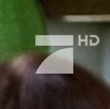
\includegraphics[width=3.5cm]{assets/images/logo_beispiel2.png} }}%
    \qquad
    \subfloat[]{{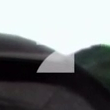
\includegraphics[width=3.5cm]{assets/images/logo_beispiel3.png} }}%
    \qquad
    \subfloat[]{{
\includegraphics[width=3.5cm]{assets/images/logo_beispiel4.png} }}%
    \qquad
    \subfloat[]{{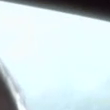
\includegraphics[width=3.5cm]{assets/images/logo_beispiel5.png} }}%
    \qquad
    \subfloat[]{{
\includegraphics[width=3.5cm]{assets/images/logo_beispiel6.png} }}%
    \caption{Logo mit verschiedenen Hintergründen}%
    \label{fig:logo5}%
\end{figure}
Eine andere Eigenschaft ist, dass bei manchen Hintergründen,
vor allem bei weissen, das Logo abgeschnitten oder kaum bis gar nicht sichtbar ist (siehe Abbildung~\ref{fig:logo5}c,d,e).
Das ist auch einfach zu erklären.
Wenn man für $a = 1$ (weiss) in die Formel oben einsetzt, erhält man: $f(1, b) = 1$,
was bedeutet, dass jeder Pixel der vorher weiss war, weiss bleibt und so das Logo nicht mehr erkennbar ist.
Analog dazu, wenn man für $a = 0$ (schwarz) einsetzt, erhält man: $f(0, b) = b$, was bedeutet, dass sich das Logo bei einem schwarzen Hintergrund
im ursprünglichen Zustand befindet.
Aus dem Grund kann das Logo komplett herausfiltert und wiederverwenden werden, wenn das Logo auf einem schwarzen Hintergrund ist (siehe Abbildung~\ref{fig:logo5}f).

\section{Werbung erkennen mithilfe des Logos}
Um ein Netzwerk zu trainieren braucht es sehr viele Daten, die kategorisiert sind.
Eine Möglichkeit, diese zu beschaffen, wäre die Bilder von Hand zu kategorisiert,
Das Problem dabei ist, dass es eine sehr langwierige und sehr langweilig Arbeit wäre,
da es um die Millionen Bilder bräuchte.
Die andere Möglichkeit ist die Bilder selber zu generieren,
indem das Logo, welches auf einem schwarzen Hintergrund ist, auf viele unterschiedliche Bilder darauf multipliziert wird.
Die unterschiedlichen Bilder erhält man aus dem Open Images Dataset V3\cite{openimages}, welches um die 9 Millionen Bilder enthält.
Da diese Bilder des Open Images Dataset nicht in der richtigen Grösse vorhanden sind, werden sie in mehrere Bilder zerteilt, welche die richtige Grösse haben.
Die Bilder könnten auch auf die richtige Grösse skaliert werden.
Das Problem dabei ist, dass dadurch viel weniger Bilder pro Sekunden erzeugt werden können und dass es den ganzen Prozess des Lernens deutlich verlangsamen würde.

Das Logo kann nun mit dem Bild negativ multipliziert werden, so dass das Logo an einem zufälligen Ort auf dem Bild erscheint (siehe Abbildung~\ref{fig:logo8}).
Man könnte sich auch überlegen, ob man das Logo nur an Position einspielt, wo es auch im Sender vorkommt.
Aber für ein convolution Netzwerk spielt es keine grosse Rolle und ausserdem hält es den Algorithmus allgemeiner.
\begin{figure}[h]%
    \centering
    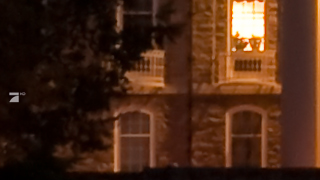
\includegraphics[width=6cm]{assets/images/logo_on_random_image.png}%
    \caption{Selbst generiertes Bild mit einem Prosieben Logo}%
    \label{fig:logo8}%
\end{figure}
Die Grösse von einem Bild ist 320x180 Pixel, da ein grösseres Bild unnötig viele Informationen enthält,
was dazu führt, dass das Netzwerk länger lernen müsste.
Ein kleineres Bild, würde das Logo noch kleiner machen und kaum noch erkennbar (siehe Abbildung~\ref{fig:logo6}).
\begin{figure}[h]%
    \centering
    
\includegraphics[width=5cm]{assets/images/logo17x11.png}%
    \caption{Prosieben Logo (17x11), extrahiert aus einem 320x180 Bild}%
    \label{fig:logo6}%
\end{figure}
Ausserdem werden die Bilder dem Netzwerk als schwarz-weiss Bild gegeben,
da man ohne Farben keinen grossen Verlust von wichtigen Informationen hat.
Und die Farben würden die Trainingsdauer ziemlich erhöhen,
da das Netzwerk viel mehr lernen müsste.
\section{Werbung erkennen ohne Hilfe des Logos}
Um Werbung zu erkennen ohne ein Logo braucht es richtige Bilder vom Sender, da Bilder von Werbung nicht einfach generiert werden können.
Da das Kategorisieren von Hand zu lange brauchen würde, wird das neuronale Netzwerk, das mithilfe des Logo die Werbung erkennt, benutzt,
um die Bilder zu kategorisieren.
Ein Problem dabei ist, dass das Netzwerk nicht perfekt ist,
um das ein bisschen auszugleichen wird die durchschnittliche\footnote{Mit Durchschnitt ist nicht der Mittelwert gemeint} Vorhersage des Netzwerks genommen,
da Werbung bzw. das normale Programm immer am Stück läuft.

Damit sichergestellt ist, dass das neue Netzwerk nicht wieder das Logo erkennt sondern die Werbung,
wird das Bild so zugeschnitten, dass das Logo nicht mehr auf dem Bild vorhanden ist.

Ausserdem werden die Bilder auch als schwaz-weiss Bild dem Netzwerk gegeben.


\chapter{Umsetzung}
\label{ch:umsetzung}
Der ganze Code kann auf Github unter https://github.com/GeorgOhneH/WerbeSkip gefunden werden.
Die verwendete Programmiersprache ist Python 3\cite{python}.
\section{Neuronales Netzwerk}
Der Code für diesen Teil befindet sich im Ordner \textit{deepnet}.\bigskip\\
Das neuronale Netzwerk ist Objekt orientiert implementiert um leicht neue Schichten und Funktionen hinzuzufügen.
Die Benutzerschnittstelle ist angelegt an Keras\footnote{eine Bibliothek für neuronale Netzwerke}.
Als Grundbaustein wird NumPy\cite{numpy}\footnote{ein Bibliothek für wissenschaftliche Datenverarbeitung} benutzt.
Da die Geschwindigkeit ein entscheidender Punkt ist, wurde alles als Matrizenmultiplikation implementiert.

\subsection{Aufbau}
\paragraph{Schichten}
Jeder Type von Schicht ist als eine Klasse implementiert, welche von einer Basisklasse erbt.
Somit kann jede Schicht gleich behandelt werden.
Jede Schicht implementieren jeweils den vorwärts und den rückwärts (backpropagation) Gang des Netzwerks.
Die Schichten sind unabhängig voneinander, bekommen aber immer die Ausgabe der vorigen Schicht bzw. der hintern Schicht bei der backpropagation.
Ausserdem sind die Aktivierungsfunktionen auch als Schicht implementiert.
\paragraph{Kostenfunktionen}
Jede Kostenfunktion ist auch eine Klasse und erbt auch von einer Basisklasse.
Jede Kostenfunktion benötigt die Implementation der Funktion und deren Ableitung.
\paragraph{Optimierer}
Ein Optimierer enthält die Funktionen für des gradient descent bzw. eine Variante davon,
da es gewisse Varianten des gradient descent gibt, die den Prozess des Lernens noch beschleunigen können,
z.B wird noch ein Impuls in den gradient descent mit einbezogen\cite{optimization}.
Auch die optimierer Klasse erbt von einer Basisklasse.
Der Optimierer wird an jede Schicht weiter geleitet um die Gewichte und Biases in der Schicht anzupassen.
\paragraph{Netzwerk}
Dies ist die Hauptklasse, es ist die Benutzerschnittstelle und
steuert die Schichten, Kostenfunktionen und Optimierer.
Ausserdem implementiert die Klasse noch diverse Funktionen, die zur Auswertung des neuronale Netzwerks hilfreich sind.

\subsection{Benutzung}
Beispiele können unter \textit{deepnet/examples} gefunden werden.\bigskip\\
Um das Programm zu benutzen müssen zuerst die Dimensionen der Eingabe bestimmen werden.
Dies würde der eingabe Schicht von einem neuronalen Netzwerk entsprechen.
Bei einem Netzwerk aus völlig verbundenen Schichten ist es die Anzahl der Neuronen.
Wenn es ein convolution Netzwerk ist, dann bestehten die eingabe Dimensionen aus 3 Zahlen.
Die erste Zahl ist die Anzahl feature map, welche der Anzahl Farbkanäle im einem Bild entsprächen würde.
Die zweite ist die Höhe des Bildes und die dritte ist die Breite des Bildes.
Danach müssen die verschiedenen Schichten bestimmt werden, darunter sind auch die Aktivierungsfunktionen.
Als nächstes muss die Kostenfunktion und der Optimierer definiert werden.
Am Schluss muss das neuronale Netzwerk noch trainiert werden, indem die Trainingsdaten dem Netzwerk gegeben werden.
Die Trainingsdaten müssen ein NumPy array sein mit der gleichen Form wie die eingabe Dimensionen mit dem Unterschied,
dass der NumPy array an der ersten Stelle eine weiter Dimension hat, welcher die Trainingsdaten enthält.
Die Trainingsdaten können auch als Generator\footnote{Ein Generator übergibt die Daten in kleinen Portionen} übergeben werden,
falls nicht genug Arbeitsspeicher vorhanden ist.

\subsection{Grafikkartenunterstützung}
Der Code kann unter \textit{numpywrapper} gefunden werden.\bigskip\\
Die Geschwindigkeit des Programmes spielt eine entscheidende Rolle für ein
neuronales Netzwerk und die Geschwindigkeit der CPU\footnote{Central processing unit} ist nicht ausreichend.
Um die GPU\footnote{Grafikkarte} zu benutzen, wird Cupy verwendet.
Da Cupy genau die gleichen Funktionen wie NumPy hat, kann es einfach mit NumPy ausgetauscht werden.
Dazu wird ein selbst geschriebenes Modul verwendet um einfach zwischen beide hin und her zuschalten.
Die GPU ist schneller als die CPU, da alles mithilfe von Matrizenmultiplikation implementiert ist und
die GPU auf Matrizenmultiplikation optimiert ist.
Das kann die Berechnungen auf meinem
PC\footnote{Auf die Hardware des PC wird in Kapitel~\ref{ch:ergebnisseUndAuswertung} näher eingegangen} um das 7-fache beschleunigen.

\subsection{Bildbearbeitung}
Der Code kann unter \textit{helperfunctions/image\_processing} gefunden werden.\bigskip\\
Der Ordner enthält die Funktionen für die Beschaffung und Formatierung der Bilder.
Um die Bilder zu dekodieren wird OpenCV\cite{opencv_library}\footnote{Bibliothek von Funktionen um Bilder zu bearbeiten} und
für die Formatierung der Bilder wird NumPy verwendet.

Die grösste Herausforderung war die Beschaffung der live stream Bilder von einem Sender.
Um die Bilder des Senders zu erhalten, wird der Teleboy Stream angezapft, nach dem Beispiel von Github\cite{gittele} und
der Stream wird durch ffmpeg\footnote{Programm für das Aufnehmen, Konvertieren und Streamen von Audio und Video} dekodiert.

\section{Webserver}
Der Code kann unter \textit{src}, \textit{app} und \textit{vuedj} gefunden werden.\bigskip\\
Um das fertige Programm zu benutzen wird eine Webseite verwendet, die unter der URL \textit{www.werbeskip.com} erreichbar ist.
Für das Backend wird Django\cite{django}\footnote{Ein web Framework} und Django Channels\cite{django_channel} verwendet, wodurch ein Websocket benutzt werden kann.
So bleibt die Verbindung mit dem Server offen und die Seite ist immer auf dem aktuellen Stand.

Für das Frontend wird VueJs\cite{vuejs} und VuetifyJS\cite{vuetify} verwendet und die Webseite ist eine Single Page Application.

\chapter{Ergebnisse und Auswertung}\label{ch:ergebnisseUndAuswertung}
Alle Berechnungen wurden auf einem PC mit einer Intel i5-4690 CPU (3.50GHz) und einer NVIDIA GeForce RTX 2070 GPU (8 GB) durchgeführt.
\section{Auswertung}
\subsection{Datensatz}\label{subsec:datensatz}
Um die Leistung der Netzwerke richtig auszuwerten wird ein selbst erstellter Datensatz verwendet,
welcher aus insgesamt 7830 Prosieben Bildern besteht.
Aus den 7830 Bildern sind 4495 Bilder mit Logo und ohne schwarzen Rand (siehe Abbildung~\ref{fig:all_logo}a),
813 mit Logo und einem oberen und unteren schwarzen Rand (siehe Abbildung~\ref{fig:all_logo}b),
813 mit Logo und einem schwarzen Rand auf beiden Seiten (siehe Abbildung~\ref{fig:all_logo}c)
und 2095 Bilder ohne Logo und ohne Rand (siehe Abbildung~\ref{fig:all_logo}d).
Ausserdem enthält der Datensatz noch 400 Bilder, die ein spezielles Prosieben Logo auf dem Bild haben (siehe Abbildung~\ref{fig:all_logo}e)
und normalerweise exkludiert sind ausser sie werden explizit erwähnt.
\begin{figure}[h]%
    \centering
    \subfloat[Normales Logo]{{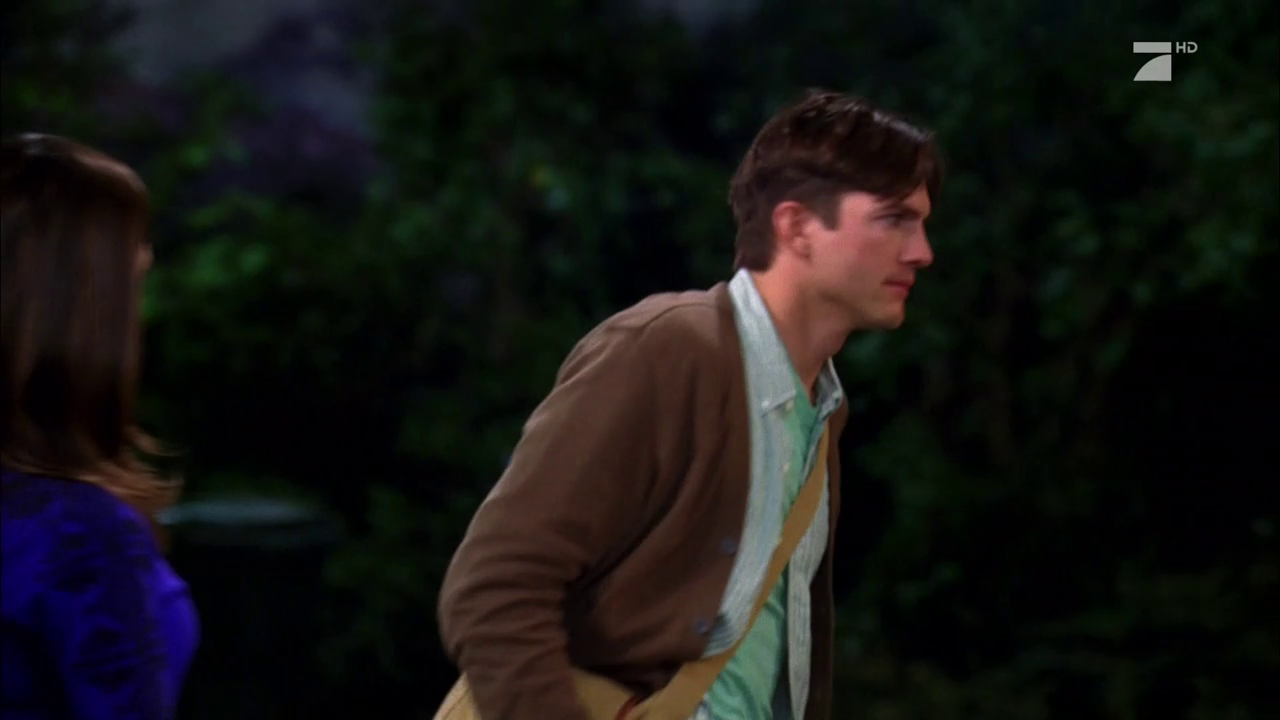
\includegraphics[width=4.5cm]{assets/images/logo_no_boarder.png} }}%
    \qquad
    \subfloat[Horizontaler Rand]{{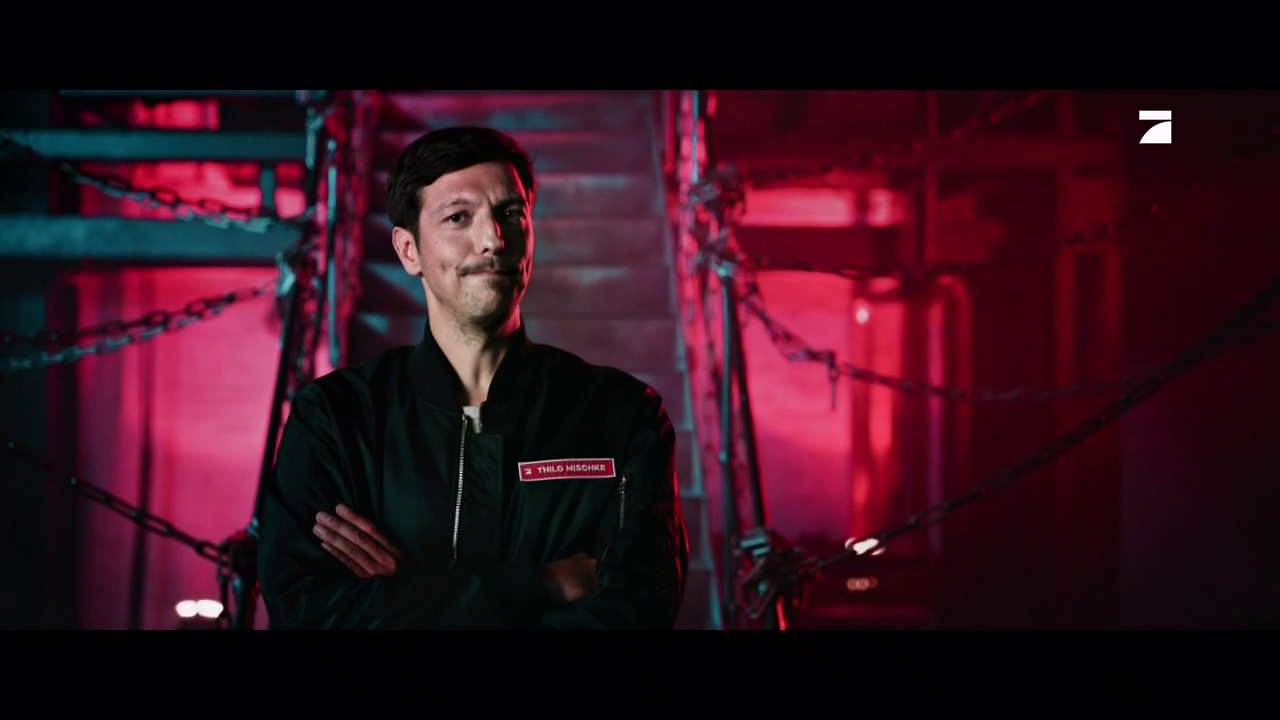
\includegraphics[width=4.5cm]{assets/images/logo_boarder_above.png} }}%
    \qquad
    \subfloat[Vertikaler Rand]{{
\includegraphics[width=4.5cm]{assets/images/logo_boarder_side.png} }}%
    \qquad
    \subfloat[Ohne Logo]{{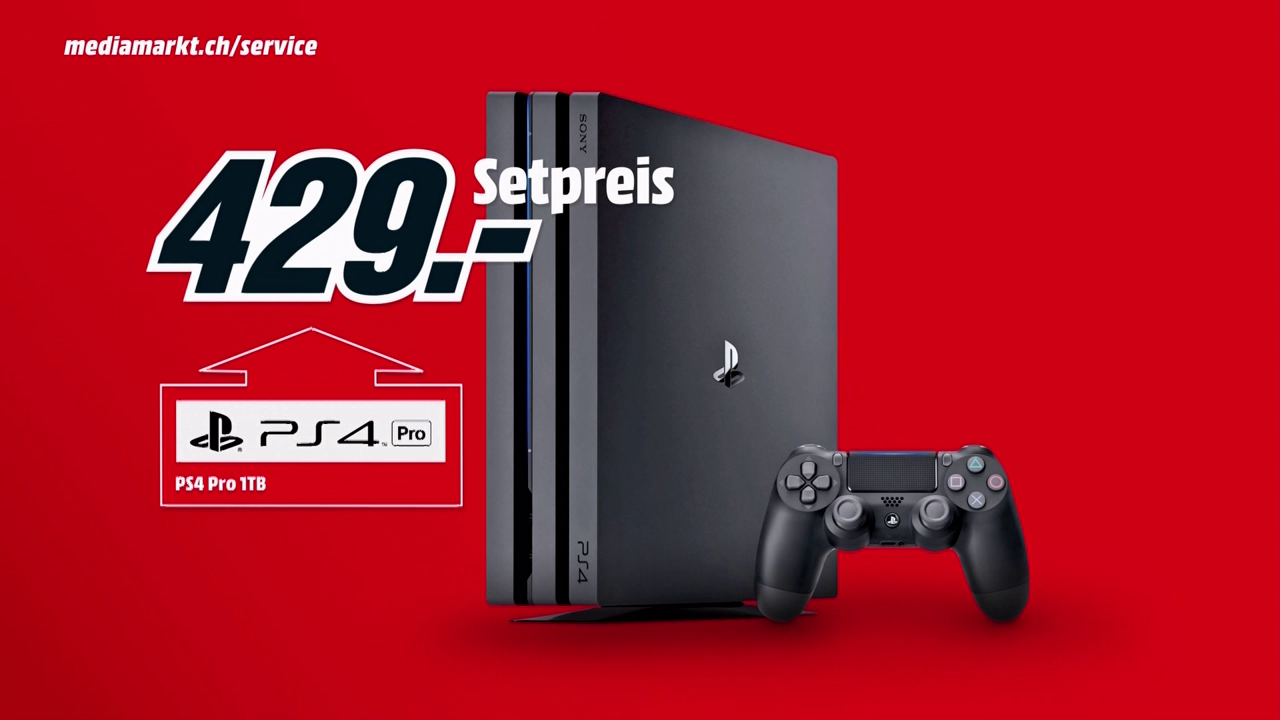
\includegraphics[width=4.5cm]{assets/images/prosieben_kein_logo.png} }}%
    \qquad
    \subfloat[Spezielles Logo]{{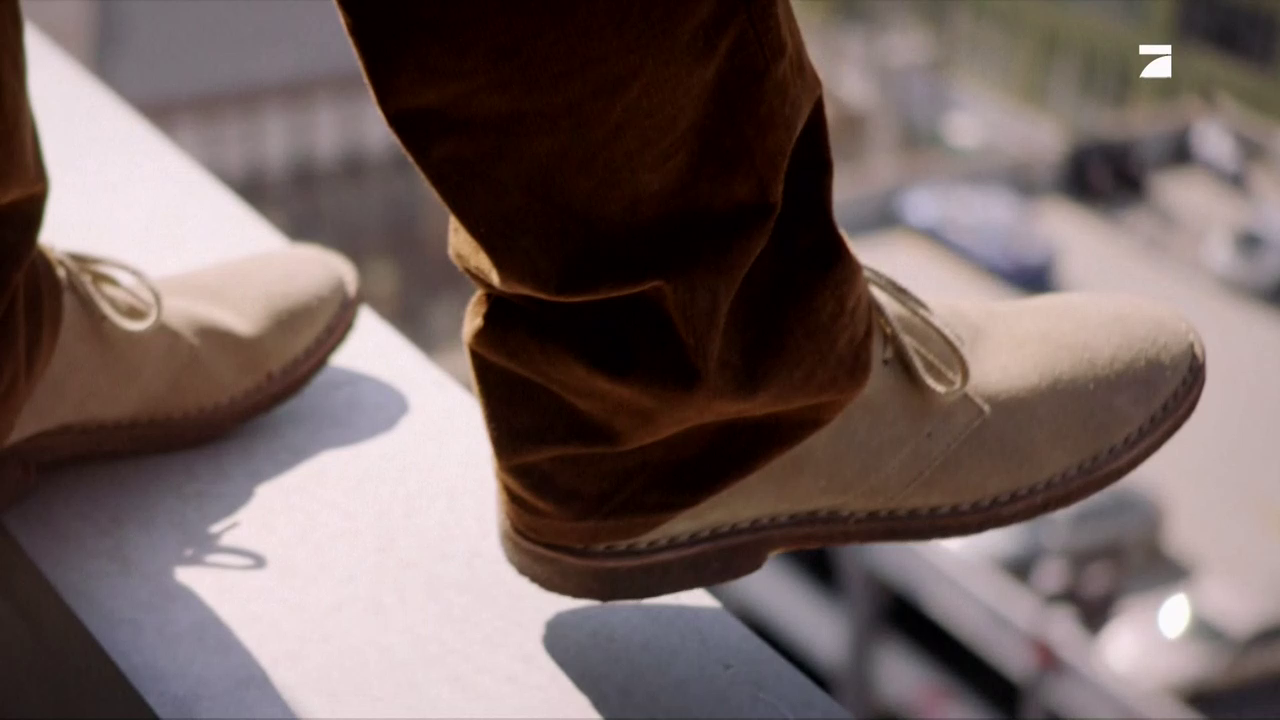
\includegraphics[width=4.5cm]{assets/images/logo_special.png} }}%
    \caption{Verschiedene Arten von Bildern im Datensatz}%
    \label{fig:all_logo}%
\end{figure}
\subsection{Methoden}
\paragraph{loss:} Die einfachste Methode das Netzwerk auszuwerten ist den Wert der Kostenfunktion anzuschauen, welcher als \textit{loss} bezeichnet wird.
Je kleiner der loss ist umso besser ist das Netzwerk.

\paragraph{Genauigkeit:} Die Genauigkeit gibt Auskunft über den Anteil der richtig erkannten Bilder.
Sie wird berechnet, indem die Anzahl richtig erkannter Bilder durch die totale Anzahl Bilder geteilt wird.
Das Problem bei der Genauigkeit und beim loss ist, dass sie nicht sehr aussagekräftig sind,
sobald der Datensatz nicht ausgeglichen ist.
Zum Beispiel hat man ein Datensatz von 100 Bildern, 90 von den Bildern haben ein Logo und 10 haben keins.
Wenn jetzt ein neuronales Netzwerk immer sagt, dass ein Logo auf dem Bild ist, ergebe das eine Genauigkeit von 90\%.
Das sieht nach einem gutes Ergebnis aus, aber das Netzwerk ist im Grunde nutzlos, da es das Logo nicht erkennt,
sondern immer nur die gleiche Ausgabe ausgibt.

\paragraph{Matthews correlation coefficient:} Der Matthews correlation coefficient\cite{wiki:mcc} behebt genau dieses Problem.
MCC\footnote{Matthews correlation coefficient} unterscheidet nicht nur zwischen falschen und wahren Vorhersagen des Netzwerk,
sondern auch zwischen wahr positiv, wahr negativ, falsch positiv und falsch negativ (Siehe Tabelle~\ref{table:mcc}).
Dadurch können verschiedene Datensätze miteinander verglichen werden, selbst wenn die Kategorien eine andere Verteilung haben\cite{wiki:mcc}.
\begin{table}[h]
    \centering
\begin{tabular}{cc|c|c|}
\cline{3-4}
                                                                                                        &                                                                           & \multicolumn{2}{c|}{Wahrer Zustand} \\ \cline{3-4}
                                                                                                        &                                                                           & Zustand positiv   & Zustand negativ \\ \hline
\multicolumn{1}{|c|}{\multirow{2}{*}{\begin{tabular}[c]{@{}c@{}}Vorausgesagt\\ Bedingung\end{tabular}}} & \begin{tabular}[c]{@{}c@{}}Vorhergesagter\\  Zustand positiv\end{tabular} & wahr positiv  & falsch positiv  \\ \cline{2-4}
\multicolumn{1}{|c|}{}                                                                                  & \begin{tabular}[c]{@{}c@{}}Vorhergesagter\\ Zustand negativ\end{tabular}  & falsch negativ    & wahr negativ   \\ \hline
\end{tabular}

\caption[Verwirrungsmatrix]{Verwirrungsmatrix}
    \small\textsuperscript{Tabelle von Wikipedia\cite{wiki:mcc}}
\label{table:mcc}
\end{table}

MCC gibt einen Wert von -1 bis +1 zurück.
Der Wert +1 repräsentiert eine perfekte Vorhersage,
0 nicht besser als eine zufällige und -1 eine komplette Unstimmigkeit zwischen Netzwerk und dem Datensatz.
Der MCC wird nach folgender Formel berechnet\cite{wiki:mcc}:
\[MCC = \frac{WP \cdot WN - FP \cdot FN}{\sqrt{(WP+FP)(WP+FN)(WN+FP)(WN+FN)}}\]
wobei WP die Anzahl der wahr positiven ist, WN die Anzahl der wahr negativen,
FP die Anzahl der falsch positiven und FN die Anzahl der falsch negativen.

\section{Neuronales Netzwerk mithilfe des Logos}
\subsection{Architektur}
Die gewählte Architektur orientiert sich am AlexNet\cite{alex}.
Es benutzt wie das AlexNet 5 convolution Schichten und benutzt nach jeder convolution und völlig verbundene
Schicht die RelU Aktivierungsfunktion.
Maxpooling wird weniger häufig angewendet als beim AlexNet, da es heute nicht mehr so üblich ist\cite{conv} und
es werden relativ kleine Werte für Dropout genommen, da genug Daten vorhanden sind und dadurch overfitting kein grosses Problem darstellt.
Ausserdem wird in jeder Schicht Batch Normalization verwedent nach dem Beispiel vom ResNet\cite{conv}.

Die letzte Schicht beinhaltet 2 Neuronen und die softmax Aktivierungsfunktion.
Das erste Neuron steht für das fehlen des Logo, wobei 0 für falsch steht und 1 für wahr.
Analog dazu steht das zweite Neuron für das vorhanden des Logo.
Durch diese zwei Neuronen und der softmax Aktivierungsfunktion kann die Ausgabe als Wahrscheinlichkeitsverteilung verstanden werden.

Das neuronale Netzwerk wurde mithilfe des \textit{Adam} Optimierers\cite{adam} und einer learning rate von 0.001 trainiert.
Der Adam Optimierer wird benutzt, da er die learning rate adaptiv anpasst und er als einer der besseren Optimierer gilt\cite{adam}.
Die learning rate sollte am Anfang vom Training relativ gross sein und am Schluss eher klein, da man am Anfang schnell in die Nähe eines Minimums kommen will
und am Schluss will man nicht über das Minimum springen.
Theoretisch könnte während dem Training die learning rate manuel angepasst werden, aber der Optimierer macht dies oft einfacher und besser.

Für die Kostenfunktion wird nicht wie im Kapitel~\ref{ch:neuronalesNetzwerk} die quadratische genommen,
sondern die \textit{cross-entropy}\cite{softmax}, welche grundsätzlich gleich funktioniert wie die quadratische, mit dem Unterschied,
dass es die Implementierung vereinfacht, da es einiges mathematisch vereinfacht\cite{softmax}.

\subsubsection{Genaue Architektur}

\begin{enumerate}
    \setlength\itemsep{0cm}
    \setlength{\parskip}{0pt}
    \setlength{\parsep}{0pt}
    \item Convolution, Anzahl Filter: 16, Filterbreite: 12, Filterhöhe: 8, Schrittweite: 4
    \item BatchNorm
    \item ReLU
    \item Convolution, Anzahl Filter: 64, Filterbreite: 6, Filterhöhe: 4, Schrittweite: 1
    \item BatchNorm
    \item ReLU
    \item Maxpool, Filterbreite: 3 Filterhöhe: 3, Schrittweite 2
    \item Convolution, Anzahl Filter: 128, Filterbreite: 4, Filterhöhe: 4, Schrittweite: 1
    \item BatchNorm
    \item ReLU
    \item Convolution, Anzahl Filter: 256, Filterbreite: 3, Filterhöhe: 3, Schrittweite: 2
    \item BatchNorm
    \item ReLU
    \item Convolution, Anzahl Filter: 512, Filterbreite: 3, Filterhöhe: 3, Schrittweite: 1
    \item BatchNorm
    \item Dropout 20\%
    \item Völlig verbundene Schicht, Neuronen: 2048
    \item BatchNorm
    \item ReLU
    \item Dropout 20\%
    \item Völlig verbundene Schicht, Neuronen: 2
    \item Softmax
\end{enumerate}

\subsection{Training}
Das Training des Netzwerks wurde nach ungefähr 17 Stunden abgebrochen, da es sich kaum noch verbessert hat.
Insgesamt wurden 2'540'000 verschiedene Bilder verwendet.
Abbildung~\ref{fig:loss1} zeigt den durchschnittlichen loss und MCC
des Netzwerks im Verlaufe des Trainings.
\begin{figure}[h]%
    \centering
    \subfloat[][loss]{{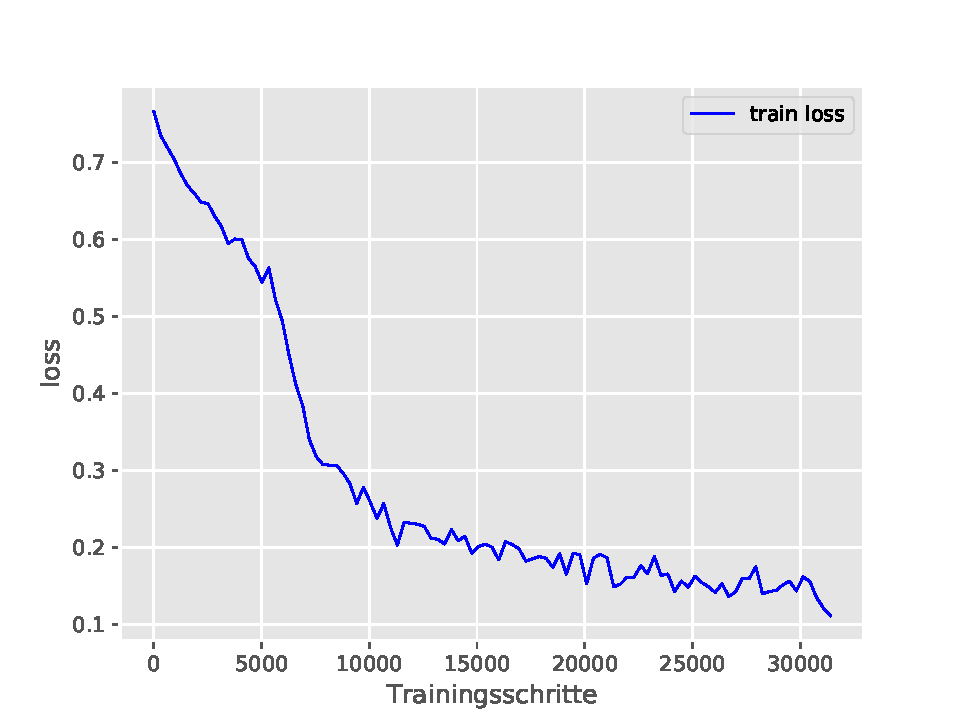
\includegraphics[width=7.5cm]{assets/images/logo_loss.pdf} }}%
    \qquad
    \subfloat[][MCC]{{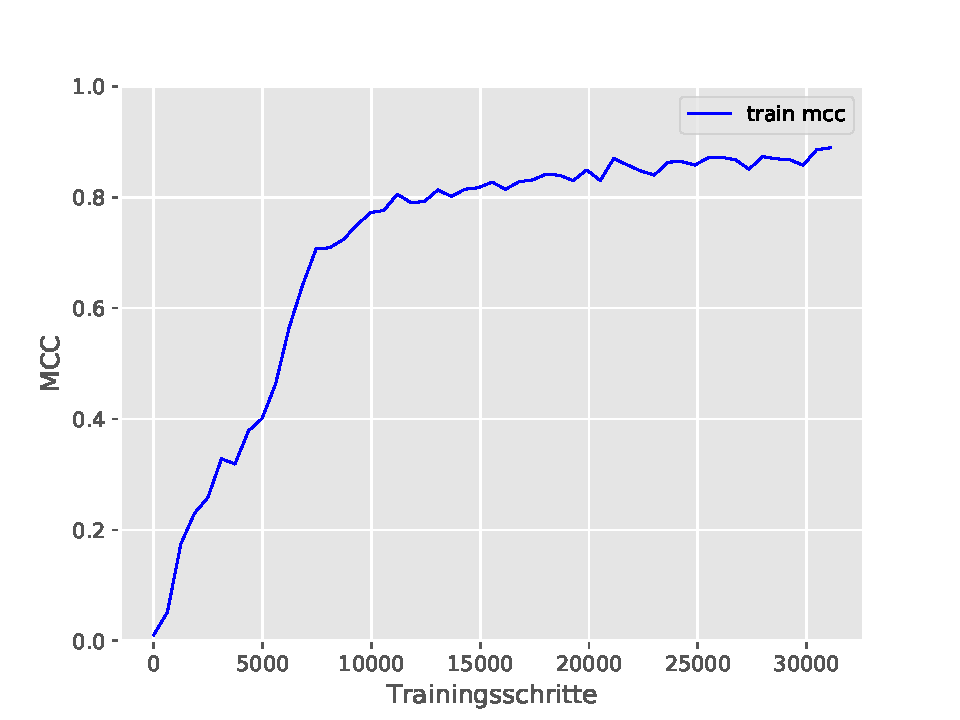
\includegraphics[width=7.5cm]{assets/images/logo_mcc.pdf} }}%
    \caption{loss und MCC im Verlaufe des Trainings}%
    \label{fig:loss1}%
\end{figure}
\subsection{Auswertung}
\subsubsection{Datensatz}
Wenn man 161'400 selbst generierte Bilder mit dem trainierten Netzwerk kategorisiert, dann erhält man durchschnittlich einen loss von 0.155,
eine Genauigkeit von 93.1\% und ein MCC von 86.7\%.
Mit dem selbst erstellten Datensatz, der in Abschnitt~\ref{subsec:datensatz} erwähnt wurde,
erhält man einen loss von 0.22, eine Genauigkeit von 91.6\% und einen MCC von 80.2\%.
Der loss und die Genauigkeit des Datensatzes und der selbst generierten Bilder sind nicht miteinander vergleichbar,
da die Verteilung der Bilder anders sind.
Die selbst generierten Bilder haben zu 50\% kein Logo und zu 50\% ein Logo.
Der Datensatz hingegen hat zu 27\% kein Logo und zu 73\% ein Logo.

Der Datensatz schneidet beim MCC um 6.5\% schlechter ab, als der MCC bei den selbst generierten Bildern.
Das könnte daran liegen, dass im Fernsehen oft noch neben dem Logo auch andere Einblendungen sind (siehe Abbildung~\ref{fig:einblenden})
und das Netzwerk diese Art von Bildern noch nie gesehen hat.
\begin{figure}[h]%
    \centering
    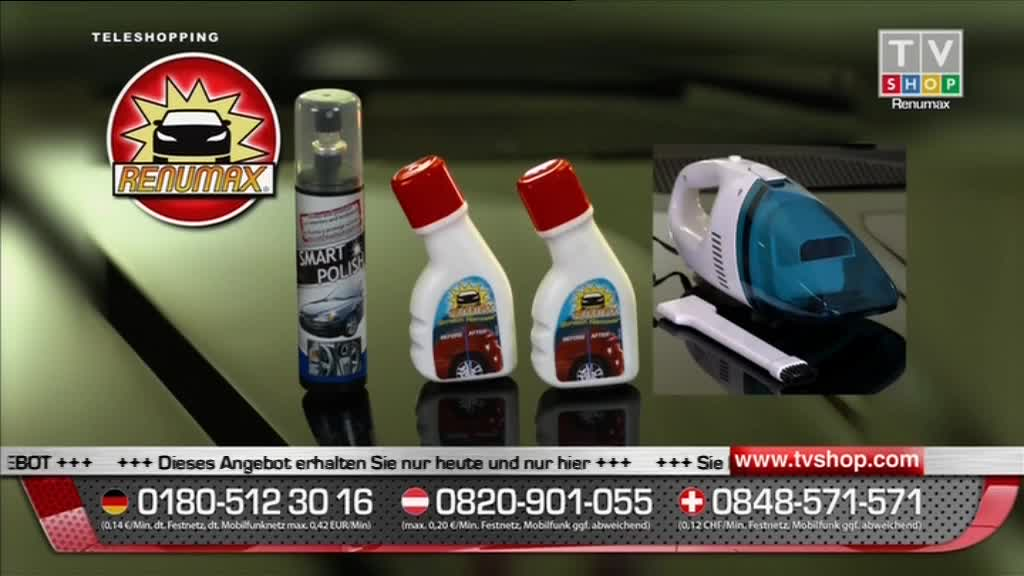
\includegraphics[width=7cm]{assets/images/tv_einblenden.jpg}%
    \caption{Einblendungen im Fernsehen}%
    \label{fig:einblenden}%
\end{figure}
Aber es ist nicht klar, ob es an den Einblendungen liegt.
Es könnte genau so gut daran liegen,
dass im Fernsehen öfters weisse Bilder vorkommen.
Das Netzwerk kann die Logos mit weissem Hintergrund schwerer kategorisieren.
Genau das ist ein grosses Problem bei einem neuronalen Netzwerk.
Eigentlich hat man keine Ahnung wie das Netzwerk genau funktioniert und wie es zu seinen Resultaten kommt.
\subsubsection{Spezielles Logo}
Wenn man von dem Datensatz nur die Bilder ohne Logo und die Bilder mit dem speziellen Logo (siehe Abbildung~\ref{fig:white_square}a) auswertet,
erhält man einen MCC von 78.2\%, welcher nur 2.0\% unter dem Wert von den normalen Bildern ist.
Das ist ziemlich überraschend, da das Netzwerk diese Art von Logo noch nie gesehen hat und trotzdem so ein gutes Resultat erzielt.

Das spezielle Logo ist fast komplett weiss und ein bisschen kleiner als das normale.
Man könnte nun denken, dass das Netzwerk nicht unbedingt das Logo erkennt,
sondern nur eine kleine weisse Stelle auf dem Bild (siehe Abbildung~\ref{fig:white_square}b).

\begin{figure}[h]%
    \centering
    \subfloat[][generiertes Bild mit dem speziellen Prosieben Logo]{{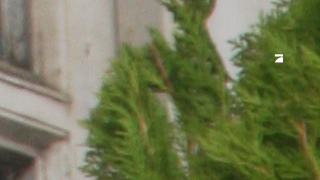
\includegraphics[width=7.5cm]{assets/images/special_logo_gen.png} }}%
    \qquad
    \subfloat[][generiertes Bild mit einer weisser Stelle (8x9)]{{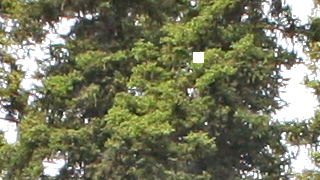
\includegraphics[width=7.5cm]{assets/images/white_square.png} }}%
    \caption{Vergleich von speziellen Logo und einer weissen Stelle}
    \label{fig:white_square}%
\end{figure}

Wenn man generierte Bildern mit dem speziellen Logo (siehe Abbildung~\ref{fig:white_square}a) durch das Netzwerk laufen lässt (natürlich auch mit Bildern ohne Logo),
erhält man mit insgesamt 207'900 Bildern einen MCC von 87.8\%,
welcher gleich gut ist, wie als wenn das normale Logo benutzt wird.
Mit generierten Bildern auf dem einer kleinen weissen Stelle ist (8x9 Pixel, die grösse des speziellen Logos)
erhält man mit insgesamt 214'000 Bildern einen MCC von 68.7\%.
Dieser Wert ist 19.1\% schlechter als wenn das spezielle Logo auf den generierten Bildern verwendet wird.
Das zeigt sehr schön, dass nicht nur die Helligkeit der Stelle entscheidend ist, sondern auch andere Faktoren, wie zum Beispiel die Form.

Auffallend ist, dass wenn man eine weisse Stelle mit der grösse von 8x8 Pixeln durch das Netzwerk laufen lässt
man mit insgesamt 160'500 Bildern einen MCC von 25.9\% erhält,
welcher massiv schlechter ist als bei der Grösse von 8x9 Pixeln.
Es zeigt, dass eine weisse Stelle eine Mindestgrösse haben muss, damit es für ein Logo gehalten werden kann.

\section{Neuronales Netzwerk ohne das Logo}
\subsection{Datenbeschaffung}
Um die Bilder von Prosieben zu kategorisieren wird das vorige neuronale Netzwerk,
welches das Logo erkennen kann, verwendet.
Die Abbildung~\ref{fig:points} zeigt die Wahrscheinlichkeit der Vorhersage des Netzwerks von live prosieben Bilder von einem gewissen Zeitraum.
Die Vorhersage ist ein Wert zwischen 0 und 1, wobei 1 für ein Vorhanden des Logos steht und 0 für kein Vorhanden des Logos.
Jeder Punkt repräsentiert eine Vorhersage.
Die Zeit ist in Sekunden angegeben und pro Sekunde hat es eine Vorhersage.
\begin{figure}[h]%
    \centering
    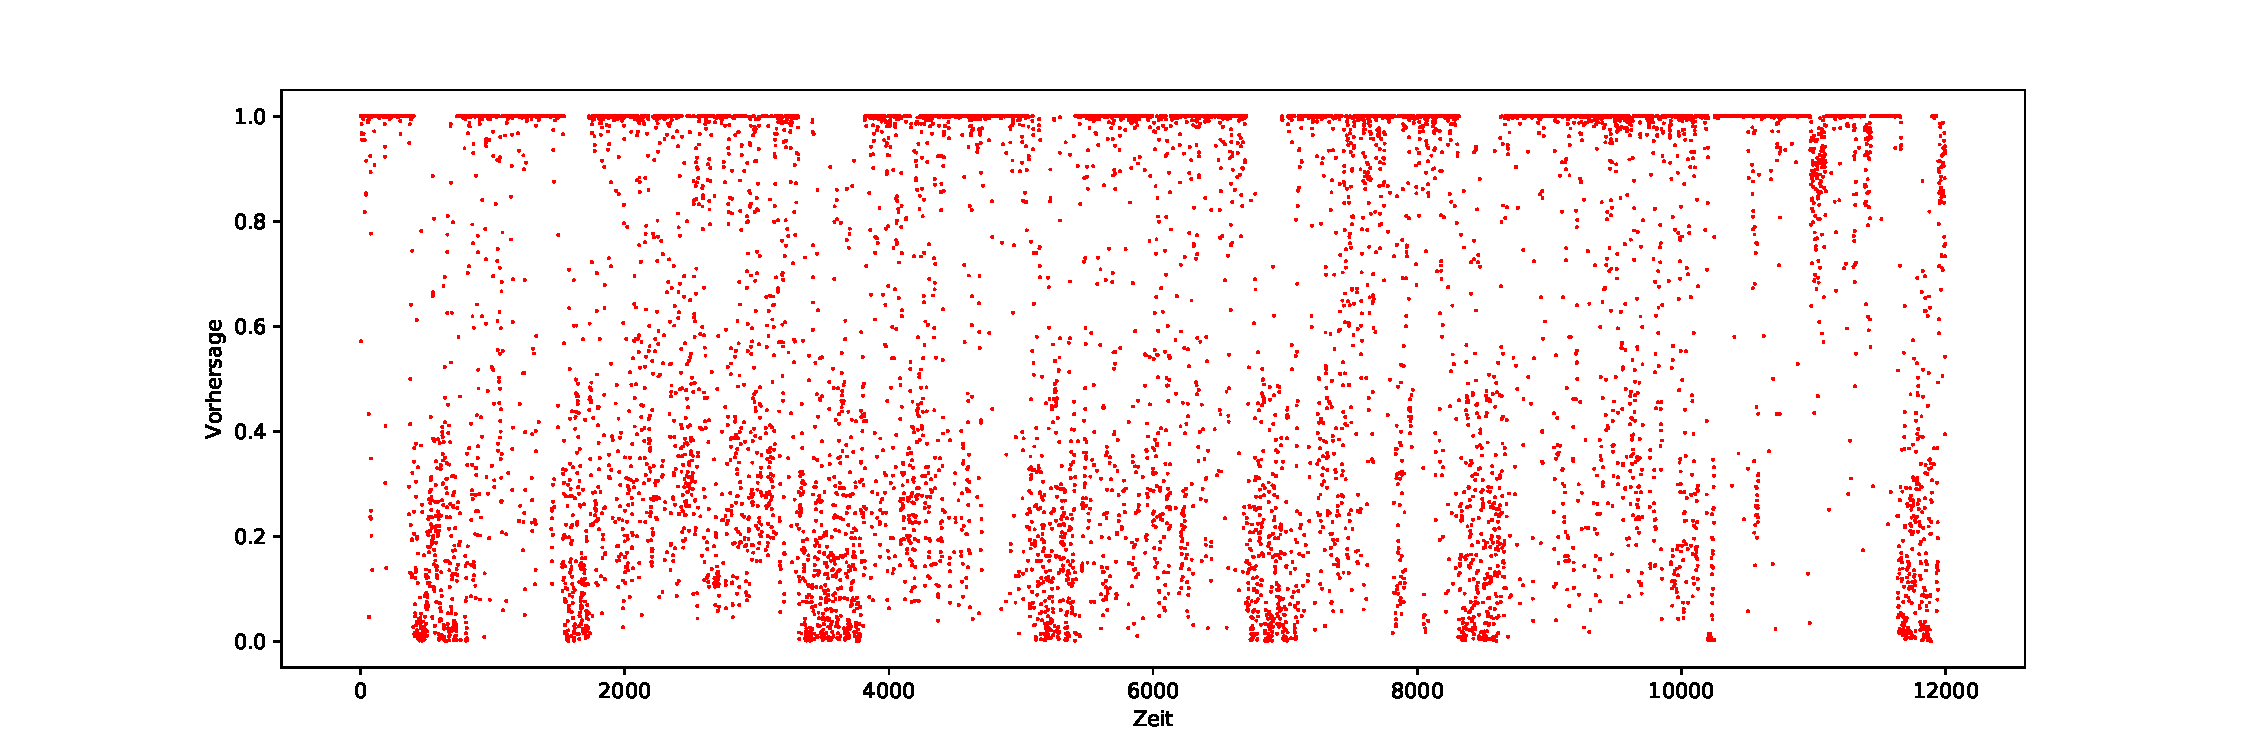
\includegraphics[width=1.0\textwidth]{assets/python/points.pdf}%
    \caption{Vorhersagen-Zeit Diagramm}%
    \label{fig:points}%
\end{figure}
Auffällig dabei ist, dass das Netzwerk viel sicherer ist, wenn es ein Logo entdeckt, als wenn es keines findet.
Das macht auch Sinn, denn wenn es keines gefunden hat, könnte das daran liegen,
dass es keines gibt oder dass das Logo nicht sichtbar ist und es eigentlich eines hat.
Dadurch kann man nur selten zu 100\% sicher sein, dass kein Logo auf dem Bild vorhanden ist.

Auf dem Diagramm können die Stellen wo Werbung lief ziemlich einfach erkannt werden.
nämlich dort, wo die obere Punktmenge, die fast wie ein Strich ausschaut, für eine längere Zeit verschwindet.
Der Algorithmus macht sich dies zur Nutze, um diese Sequenz von Bildern zu kategorisieren.
Es wird geschaut, ob in den letzten 25 Sekunden eine Vorhersage über 0.9 gewesen ist.
Wenn dies 5 mal hintereinander zutrifft, wird das Bild als keine Werbung kategorisiert.
Analog dazu müssen 5 mal hintereinander die letzten 25 Sekunden die Vorhersage unter 0.9 sein,
damit es als Werbung kategorisiert wird.
Falls beides nicht zutreffen sollte, wird das Bild gleich wie das vorige Bild kategorisiert.
Abbildung~\ref{fig:points_line} zeigt das Resultat des Algorithmus\footnote{Dieser Algorithmus wird auch von dem Webserver verwendet}.
\begin{figure}[h]%
    \centering
    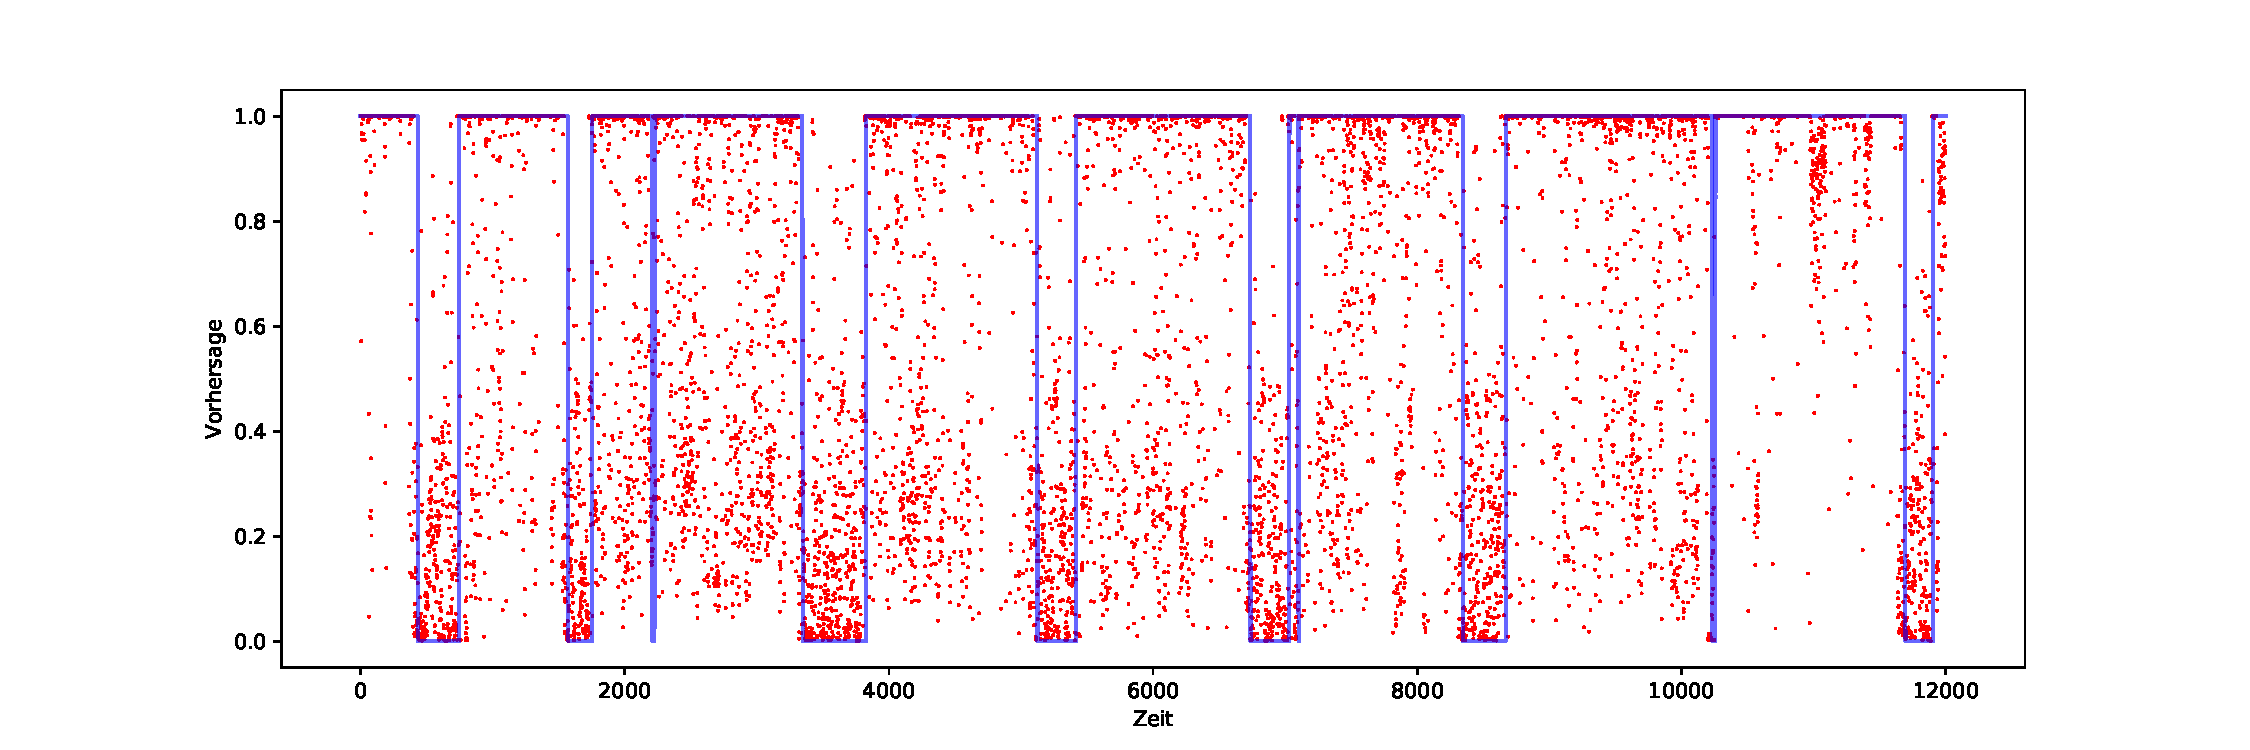
\includegraphics[width=1.0\textwidth]{assets/python/points_blue_line.pdf}%
    \caption{Vorhersagen-Zeit Diagramm mit Kategorisierung}%
    \label{fig:points_line}%
\end{figure}
Die Kategorisierung ist nicht perfekt, aber gut genug um das Netzwerk zu trainieren.
Der kleine Teil, der falsch kategorisiert ist, hat keinen grossen Einfluss auf den Trainingsprozess.

Ausserdem werden die Bilder noch zugeschnitten, so dass das Logo nicht mehr auf dem Bild vorkommt.
Die Bilder haben schliesslich eine Grösse von 269x141 Pixel (siehe Abbildung~\ref{fig:cropped_img}).
\begin{figure}[h]%
    \centering
    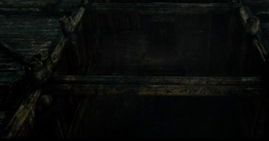
\includegraphics[width=7cm]{assets/images/cropped.png}%
    \caption{Zugeschnittenes Bild (269x141)}%
    \label{fig:cropped_img}%
\end{figure}
\subsection{Architektur}
Es wird die gleiche Architektur benutzt wie für das vorige Netzwerk mit dem Unterschied,
dass mehr Dropout verwendet wurde, da Bilder mehrmals verwendet werden.
Ausserdem sind die Parameter des Filters angepasst, da die Bilder eine andere Grösse haben und die gleichen Parameter nicht mehr funktionieren würden.
\subsubsection{Genau Architektur}

\begin{enumerate}
    \setlength\itemsep{0cm}
    \setlength{\parskip}{0pt}
    \setlength{\parsep}{0pt}
    \item Convolution, Anzahl Filter: 16, Filterbreite: 9, Filterhöhe: 9, Schrittweite: 4
    \item BatchNorm
    \item ReLU
    \item Convolution, Anzahl Filter: 64, Filterbreite: 6, Filterhöhe: 6, Schrittweite: 1
    \item BatchNorm
    \item ReLU
    \item Maxpool, Filterbreite: 3 Filterhöhe: 3, Schrittweite 2
    \item Convolution, Anzahl Filter: 128, Filterbreite: 4, Filterhöhe: 4, Schrittweite: 1
    \item BatchNorm
    \item ReLU
    \item Convolution, Anzahl Filter: 256, Filterbreite: 3, Filterhöhe: 3, Schrittweite: 2
    \item BatchNorm
    \item ReLU
    \item Convolution, Anzahl Filter: 512, Filterbreite: 3, Filterhöhe: 3, Schrittweite: 1
    \item BatchNorm
    \item Dropout 25\%
    \item Völlig verbundene Schicht, Neuronen: 2048
    \item BatchNorm
    \item ReLU
    \item Dropout 50\%
    \item Völlig verbundene Schicht, Neuronen: 2
    \item Softmax
\end{enumerate}
\subsection{Training}
Das Training des Netzwerks wurde nach ungefähr 43 Stunden abgebrochen, da es sich nicht verbessert hat.
Insgesamt wurden 339'200 Bilder durch das Netzwerk geschleust, wobei auch gleiche Bilder mehrmals verwendet worden sind.
Dieser Trainingsprozess dauerte länger und hat weniger Bilder verarbeitet, als das Netzwerk, welches das Logo erkennen kann.
Das liegt daran, dass nicht die GPU die Geschwindigkeit den Trainingsprozess begrenzt, sondern die Beschaffung der Daten.
Aus einem Livestream können nur eine begrenze Anzahl Bilder pro Sekunde extrahiert werden und dadurch verlangsamt sich den Prozess erheblich.

Abbildung~\ref{fig:loss2}a,b zeigt den durchschnittlichen loss und MCC,
des Netzwerk im Verlaufe des Trainings.
\begin{figure}[h]%
    \centering
    \subfloat[][loss]{{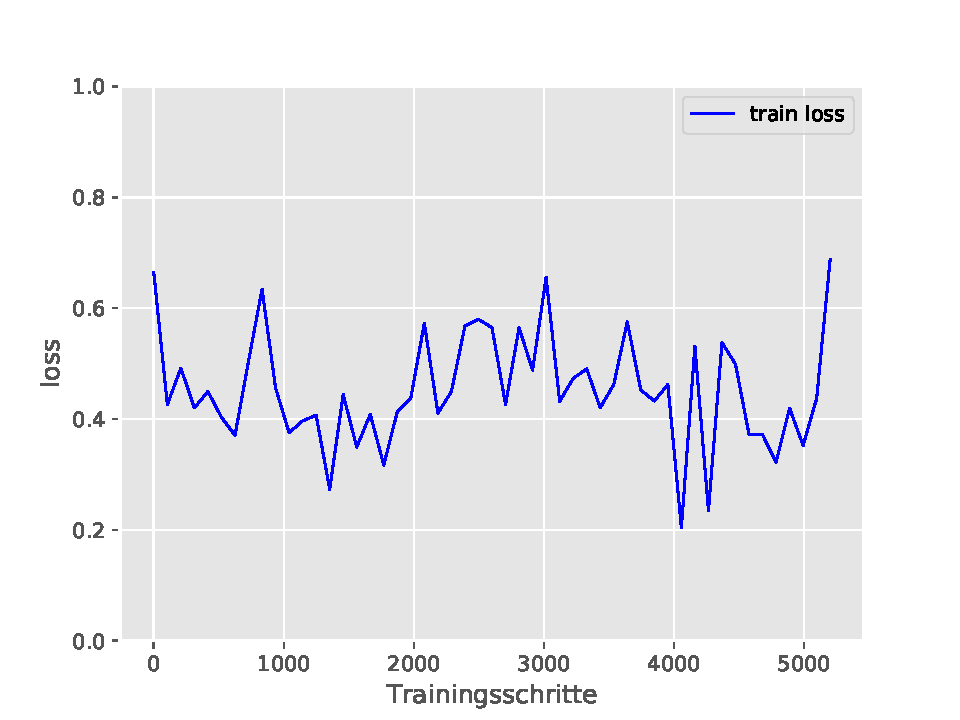
\includegraphics[width=7.5cm]{assets/images/no_logo_loss.pdf} }}%
    \qquad
    \subfloat[][MCC]{{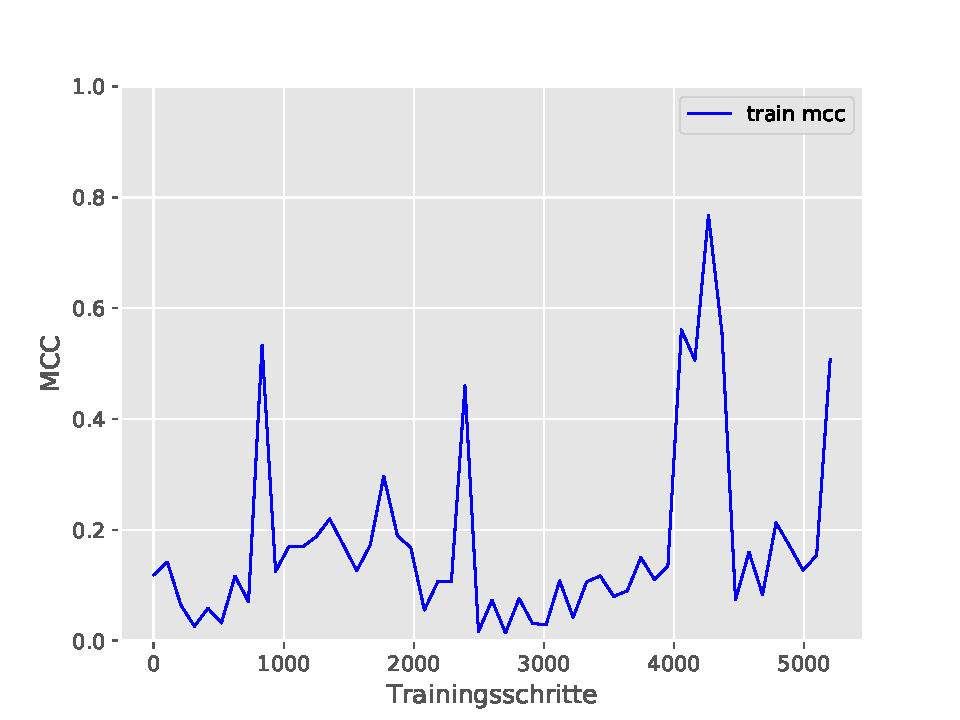
\includegraphics[width=7.5cm]{assets/images/no_logo_mcc.pdf} }}%
    \caption{loss und MCC im Verlaufe des Trainings}%
    \label{fig:loss2}%
\end{figure}
\subsection{Auswertung}
An Abbildung~\ref{fig:loss2}a,b erkennt man,
dass sich der loss und der MCC während dem Training nicht positiv verändert haben und das Netzwerk nichts viel gelernt hat.
Auch die Auswertung des Datensatzes (mit den speziellen Logos) bestätigt, dass das Netzwerk nicht viel gelernt hat.
Man erhält einen loss von 1.354, eine Genauigkeit von 37.2\% und einen MCC von 16.4\%, welche alle sehr schlechte Werte sind.
Ein zufälliges initialisiertes Netzwerk  erzielt einen loss von 1.287, eine Genauigkeit von 41.3\% und einen MCC von 15.8\%.
Das zeigt, dass das trainierte Netzwerk genauso schlecht ist wie ein zufällige initialisiertes Netzwerk.
Man kommt zum Schluss, dass das Netzwerk in keiner Weise fähig ist, die Werbung zu erkennen.

Es könnte natürlich sein, dass das Netzwerk einfacher eine kompliziertere Architektur haben muss und mehr Daten braucht um ein bessere Ergebnisse zu erbringen.
Da aber für diese Arbeit nur sehr begrenzt Ressourcen zur Verfügung stehen, kann dies nicht weiter getestet werden.


\chapter{Fazit und Weiterführung}\label{ch:fazitUndWeiterführung}
\section{Fazit}
Das Ziel in dieser Arbeit war die zu Überprüfen, ob die Erkennung von Werbung mithilfe eines neuronalen Netzwerks möglich ist.
Das Ziel wurden nur indirekt erreicht.

Es war nicht möglich einem convolution neuronalen Netzwerk beizubringen wie Werbung ausschaut und an welchen kriterien man die Werbung erkennen könnte.
Das Misslingen könnte daran liegen, dass Werbung zu ähnlich zum normalen Programm ist oder dass das Netzwerk viel komplizierter sein muss und viel mehr Daten braucht.

Hingegen war die Erkennung vom Prosieben Logo ein Erfolg.
Es war möglich mit einem convolution neuronalen Netzwerk das Prosieben Logo in jeder beliebigen Position auf einem schwarz-weissen Bild zu erkennen.
Da das Prosieben Logo nur eingespielt wird, wenn keine Werbung läuft,
kann ziemlich exakt bestimmt werden, ob Werbung läuft oder nicht.

\section{Mögliche Weiterführung}
In dieser Arbeit wurde nur ein winziger Bruchteil von Methoden für ein neuronales Netzwerk präsentiert.
Die Resultate die in der Arbeit gezeigt worden sind, können sicher noch verbessert werden.
Die Netzwerke könnten mit neueren Methoden und mehr Rechenleistung um ein Vielfaches verbessert werden.

Eine denkbare Weiterführung für das Netzwerk wäre, dass-                                                                                                                                                                                                                                                                                                                                                                                                                                                                                                                                                                                                                                                                                                                                                                                                                                                                                                                                                                                                                                                                                                                                                                                                                                                                                                                                                                                                                                                                                                                                                                                                                                                                                                                                                                                                                                                                                                                                                                                                                                                                                                                                                                                                                                                                                                                                                                                                                                                                                                                                                                                                                                                                                                                                                                                                                             es nicht nur ein Art von Logo erkennen kann, sondern auch noch andere Logos,
z.B. könnte dann ein Netzwerk nicht nur das Prosieben Logo erkennen, sondern das Prosieben Logo und das SRF Logo.

Eine andere Verbesserung könnte sein, dass man ein recurrent neuronale Netzwerke\cite{wiki:rnn} benutzen würde.
Ob Werbung in diesem Moment läuft oder nicht wird bestimmt, indem die durchschnittliche Ausgabe vom Netzwerk berechnet wird.
Ein recurrent neuronale Netzwerke wäre genau für solche Sequenzen von Daten gemacht und man könnte anstatt den Durchschnitt zu berechnen
ein recurrent neuronale Netzwerke trainieren, welches die Aufgabe sicher besser lösen würde.


\clearpage
\phantomsection
\addcontentsline{toc}{chapter}{Literaturverzeichnis}
\nocite{*}
\bibliography{C:/Jetbrains/PyCharm/WerbeSkip/thoughts/arbeit/maturaarbeit}
\bibliographystyle{plain}

\clearpage
\phantomsection
\addcontentsline{toc}{chapter}{Abbildungsverzeichnis}
\listoffigures
Abbildungen aus dem Kapitel~\ref{ch:neuronalesNetzwerk} sind von Michael A. Nielsen's Buch\cite{neuralbook} inspiriert.

\appendix


\chapter*{Ehrlichkeitserklärung}

Die eingereichte Arbeit ist das Resultat meiner persönlichen, selbstständigen Beschäftigung mit dem Thema.
Ich habe für sie keine anderen Quellen benutzt als die in den Verzeichnissen aufgeführten.
Sämtliche wörtlich übernommenen Texte (Sätze) sind als Zitate gekennzeichnet.

\vspace{2cm}
Basel, \today
\end{document}
